\documentclass[12pt,a4paper]{article}
\usepackage[margin=2.5cm]{geometry}
\usepackage{amsmath,amssymb,amsthm}
\usepackage{booktabs}
\usepackage{array}
\usepackage{multirow}
\usepackage{xcolor}
\usepackage{hyperref}
\usepackage{natbib}
\usepackage{setspace}
\usepackage{caption}
\usepackage{graphicx}
\usepackage{enumitem}
\usepackage{bm}
\usepackage{bbm}

\onehalfspacing

\newtheorem{proposition}{Proposition}
\newtheorem{corollary}{Corollary}[proposition]
\newtheorem{lemma}{Lemma}
\newtheorem{remark}{Remark}
\newtheorem{assumption}{Assumption}
\theoremstyle{definition}
\newtheorem{definition}{Definition}

% Notation shortcuts
\newcommand{\Sig}{\Sigma_e}
\newcommand{\sighat}{\hat\Sigma_e}
\newcommand{\wopt}{w^{\mathrm{opt}}}
\newcommand{\wave}{w^{\mathrm{ave}}}
\newcommand{\Qopt}{Q^{\mathrm{opt}}}
\newcommand{\Qave}{Q^{\mathrm{ave}}}
\newcommand{\Qsub}{Q_k^{\mathrm{sub}}}
\newcommand{\Qbag}{Q_k^{\mathrm{bag},\infty}}
\newcommand{\QbagG}{Q_k^{\mathrm{bag},G}}
\newcommand{\Lbag}{L_k^{\mathrm{bag},\infty}}
\newcommand{\Lsub}{L_k^{\mathrm{sub}}}
\newcommand{\Rk}{R_k^{\mathrm{bag},\infty}}
\newcommand{\vbar}{\bar{v}_k}
\newcommand{\zk}{z_k}
\newcommand{\E}{\mathbb{E}}
\newcommand{\Var}{\mathrm{Var}}
\newcommand{\Cov}{\mathrm{Cov}}

\title{\textbf{Bagged Random Subset Methods for Forecast Combination:
       Theory, Monte Carlo, and Empirical Evidence}\\[0.5em]
       \large Exact Results, Power-Law Excess Risk, and the Cube-Root Law}
\author{Boris Kozyrev}
\date{June 2026}

\begin{document}
\maketitle

\begin{abstract}
We study Random Subset Methods (RSM) for forecast combination in a panel of
$m$ individual forecasters.  The paper proceeds inductively.  We first
establish exact population results under the common-loading covariance
model: a \emph{conservation law} governing how precision-weighted RSM
weights redistribute across subsets, an exact formula for the
infinite-bagged excess risk $\Rk$, monotone decrease of $\Rk$ in $k$
(proved under a stated contraction condition, verified numerically),
and a first-order condition for the optimal subset size $k^*$.
We then show that the average-subset risk is tractable via Taylor expansion,
yielding a square-root optimal subset size $k^*_{\mathrm{sub}}\propto T^{1/2}$.
The infinite-bagged risk resists the same treatment because the key
conditional expectation has no closed form without further restrictions.
We use Monte Carlo experiments with known $\Sigma_e$ to characterise the
functional form of $\Rk$ empirically: the power-law family
$\Rk\approx Cz_k^\alpha$, $z_k=1/k-1/m$, fits with $R^2>0.97$ in all
designs.  The exponent $\hat\alpha\in(1,2)$ is determined by the
heterogeneity ratio $H$ of idiosyncratic variances and implies an optimal
subset size $k^*\propto T^{1/(\alpha+1)}$ scaling between $T^{1/3}$
(small heterogeneity, $\alpha\to 2$) and $T^{1/2}$ (dominant forecaster,
$\alpha\to 1$).  For the endogenous case (estimated $\Sigma_e$) we provide a
tractable result under strict Gaussianity and common loading via the
Kan--Zhou correction, which preserves the $T^{1/(\alpha+1)}$ scaling
exponent; the subset-level correction factor $(T-2)/(T-k-2)$ is small
for $k\ll T$ and produces only a modest level shift in $k^*$.  Empirically
the endogenous optimal $k^*$ is substantially larger than the tractable
prediction, driven by non-common-loading misspecification rather than
estimation noise per se.  Applying RSM to FRED-MD GDP forecasts yields
statistically significant RMSFE reductions of 10--30\% over the
equal-weighted mean.  The Survey of Professional Forecasters---a
near-homogeneous panel---confirms that RSM offers little advantage when
forecasters are nearly identical in quality.
\end{abstract}

\tableofcontents
\newpage

%===========================================================================
\section{Scope and Main Message}
\label{sec:scope}
%===========================================================================

The central question is: in a large panel of $m$ individual forecasters,
how many should a practitioner randomly subsample, and how should subsample
forecasts be combined, to minimise out-of-sample loss?

Two distinct RSM objects have been studied in the literature.  The
\emph{average-subset estimator} picks a random size-$k$ subset, fits
constrained OLS within it, and reports that single forecast.  The
\emph{bagged estimator} averages $G$ such draws; as $G\to\infty$ it
converges to the infinite-bagged estimator.  Since $w\mapsto w'\Sig w$ is
convex, Jensen's inequality gives
$Q_k^{\mathrm{bag},\infty}\leq Q_k^{\mathrm{sub}}$,
so bagging always weakly reduces population risk.  Yet prior work has
largely analysed $Q_k^{\mathrm{sub}}$ and assumed a functional form
for the bagged excess risk.  We derive what can be derived exactly, then
use Monte Carlo to characterise what cannot.

\paragraph{Logic of the paper.}
Sections~\ref{sec:setup}--\ref{sec:bench} establish the framework and
show that the equal-weighted mean and full estimated optimal are special
cases of RSM.  Section~\ref{sec:rsm} defines RSM and derives the
exact finite-bagging bridge.  Section~\ref{sec:cl} exploits the
common-loading structure to obtain the conservation law, exact excess-risk
formula, monotone decrease of $\Rk$, and a first-order condition for $k^*$.
Section~\ref{sec:tractable} derives the average-subset optimum and shows
why the bagged optimum resists a parallel derivation.
Section~\ref{sec:exomc} uses Monte Carlo with known $\Sigma_e$ to motivate
the power-law parametrisation of $\Rk$, characterise $\hat\alpha$, and
validate the implied $k^*$.  Section~\ref{sec:endomc} studies the
endogenous case, beginning with a tractable result under strict Gaussianity
and closing with Monte Carlo evidence for general designs.
Sections~\ref{sec:spf}--\ref{sec:gdp} present the empirical applications.

\subsection{Motivation and Relation to the Literature}
\label{sec:motivation}

\paragraph{The forecast combination puzzle and Elliott--Liao (2025).}
A long-standing puzzle in forecast combination is that the equal-weighted
mean of individual forecasts typically outperforms the estimated
minimum-variance combination, despite the latter being the solution to a
simple constrained OLS problem \citep{BatesGranger1969,GrangerRamanathan1984}.
\citet{ElliottLiao2025} provide a complementary perspective: rather than
attributing the puzzle solely to estimation error, they ask how large the
\emph{population} gains from optimal combination can be under empirically
motivated restrictions on the forecast-error covariance $\tilde\Sigma$.
Their model,
\begin{equation}\label{eq:EL_model}
  \tilde\Omega = \sigma_\varepsilon^2\bm{\iota}\bm{\iota}' + \tilde\Sigma,
\end{equation}
is precisely our common-loading structure ($q=\sigma_\varepsilon^2$,
$D=\tilde\Sigma$).  Using SPF data to discipline the space of $\tilde\Sigma$,
they show that for most empirically plausible parameterisations the population
gain $\Qave-\Qopt$ is small relative to estimation error $(m-1)/T$ ---
providing a theoretical rationale for the combination puzzle that operates
even in population, before any finite-sample noise.

\paragraph{Inflation factors: Elliott--Liao vs RSM.}
A key ingredient in the puzzle is the \emph{inflation factor} --- the
multiplier by which the in-sample optimal-combination loss exceeds its
true population value because the weights are estimated rather than known.
For the full $m$-weight optimal combination estimated by constrained OLS,
the standard degrees-of-freedom correction is
\begin{equation}\label{eq:EL_inflation}
  I_m(T) \;=\; \frac{T-1}{T-m},
\end{equation}
the exact Gaussian correction for estimating $m-1$ free parameters from
$T$ observations.  Its leading-order excess over 1 is
\begin{equation}\label{eq:EL_excess}
  I_m(T)-1 \;\approx\; \frac{m-1}{T},
\end{equation}
and it is this quantity $(m-1)/T$ that \citet{ElliottLiao2025} use as
their benchmark for the expected estimation cost.  They call it the
\emph{best case} for OLS because it is the minimum possible estimation
error: it assumes Gaussian errors, a correctly specified model, and the
full $m$-dimensional weight vector.  Any real-world estimation procedure
can only do worse.  Their criterion for full optimal combination to be
worthwhile is then $\Qave-\Qopt > (m-1)/T\cdot(\sigma_\varepsilon^2+\Qopt)$;
for most empirically calibrated $\tilde\Sigma$ this condition fails, which
they show as the rationale for the combination puzzle.

The present paper departs from this framework in a single but critical
respect: we use the inflation factor $(T-1)/(T-k)$ for a \emph{subset}
of size $k<m$, not the full-model factor $(T-1)/(T-m)$.  Since $k\ll m$,
the RSM inflation is substantially smaller:
\begin{equation}\label{eq:rsm_inflation_advantage}
  \frac{T-1}{T-k} \;\ll\; \frac{T-1}{T-m},
  \quad\text{i.e.}\quad
  \frac{k-1}{T} \;\ll\; \frac{m-1}{T}.
\end{equation}
This opens a window of viable gains that the full-model approach cannot
access: RSM can produce a net positive out-of-sample improvement even when
Elliott--Liao's benchmark says full OLS combination is not worth estimating,
because RSM's estimation cost is only $(k-1)/T$ rather than $(m-1)/T$.
Choosing $k$ optimally therefore means choosing the largest subset for
which the RSM gain $\Qave-\Qbag$ exceeds the RSM-specific inflation cost
--- the central problem this paper solves.

Their Proposition~1 gives a precise characterisation: when $\bm{\iota}$
is an eigenvector of $\tilde\Sigma$ (equivalently, all row sums of
$\tilde\Sigma$ are equal), the equal-weighted mean \emph{is} the optimal
combination and gains are exactly zero.  In our notation this corresponds
to $V_\delta=0$, hence $C_\delta=0$, the near-homogeneous case in which
$k^*=1$ (Remark~\ref{rem:flat}).

Their key positive result (Section~3.2, Proposition~2) concerns the case
where gains \emph{are} large.  They characterise the worst-case $\tilde\Sigma$
for the equal-weighted mean: the maximiser of $\Qave-\Qopt$ over the
restricted space has a block structure
$\Sigma_{11}=I_{m_1}$, $\Sigma_{12}=m_1^{-1}\iota_1\iota_2'$, and the
corresponding optimal weights are
\begin{equation}\label{eq:EL_wopt}
  w^{\mathrm{opt}} = \begin{pmatrix}(1/m_1)\,\iota_1 \\ 0\end{pmatrix}.
\end{equation}
That is: \emph{take the equal-weighted average of the first $m_1$
forecasters and discard the remaining $m-m_1$}.  This is the
Complete Subset estimator of \citet{ElliottGarganoTimmermann2013} (CSR):
a fixed subset of size $m_1$ with equal within-subset weights.  Elliott
and Liao thus establish that CSR is the \emph{optimal} response when gains
from full optimal combination are largest --- but they stop short of two
important questions: (i) which forecasters should be in the retained
subset, and (ii) how large should the subset be?

\paragraph{How RSM improves on the Elliott--Liao prescription.}
RSM addresses both gaps and goes one step further.
\begin{enumerate}[nosep,label=(\roman*)]
  \item \textbf{Subset selection via randomisation.}  Searching
    deterministically for the best size-$m_1$ subset is combinatorially
    intractable ($\binom{m}{m_1}$ candidates).  RSM replaces this with
    uniform random draws and averaging --- eliminating subset-selection
    variance without any search.
  \item \textbf{Optimal within-subset weights.}  Elliott--Liao's prescription
    uses equal weights within the retained subset.  RSM instead applies
    constrained minimum-variance OLS within each draw, giving weights
    $w_{S,i}=\tau_i/A_S$.  Since $w_S=\arg\min_{w'\iota=1}w'\Sigma_Sw$, we have
    $w_S'\Sigma_S w_S\le (1/k^2)\iota'\Sigma_S\iota$ --- optimal weights
    are always at least as good as equal weights within the same subset.
    Taking expectations over $S$:
    $Q_k^{\mathrm{RSM}}\le Q_k^{\mathrm{CSR}}$ strictly whenever $\Sigma_e$
    is not a multiple of the identity.
  \item \textbf{Optimal $k^*$.}  Neither Elliott--Liao nor CSR provide a
    theory for the optimal subset size.  The present paper derives this:
    $k^*\propto T^{1/(\alpha+1)}$ under the power-law parametrisation of
    the excess risk, with the endogenous approximation
    $k^*\approx\lfloor\sqrt{T}\rfloor$ for practical use.
\end{enumerate}

\paragraph{Chen and Maung (2023) and the cost of ad hoc $k$ selection.}
\citet{ChenMaung2023} develop nonparametric time-varying forecast combination
for high-dimensional data.  In their empirical application to inflation and
unemployment forecasting they include CSR \citep{ElliottGarganoTimmermann2013}
as a benchmark, evaluated at $k\in\{1,2,3,5\}$.  Their Table~3 reveals a
telling pattern (ASCFE ratios relative to the AR benchmark; below 1 is better):

\begin{center}
\begin{tabular}{lcccc}
\toprule
Series & $k=1$ & $k=2$ & $k=3$ & $k=5$ \\
\midrule
Inflation    & 0.98 & 0.95 & 0.93 & 0.96 \\
Unemployment & 1.01 & 1.02 & 1.01 & 0.97 \\
\bottomrule
\end{tabular}
\end{center}

For \emph{unemployment}, performance is monotonically improving through
$k=5$ --- the curve is still decreasing at the largest $k$ they consider.
For \emph{inflation}, the minimum is near $k=3$--$4$ but was never
precisely located; Chen and Maung do not study $k>5$.  In both cases they
were on the decreasing side of the U-shaped RMSFE$(k)$ curve and never
found the optimum.  The theory in this paper predicts
$k^*\approx\lfloor\sqrt{T}\rfloor\approx 10$--$12$ at the sample sizes
they used ($T\approx100$--$150$), substantially above $k=5$.

\paragraph{Relation to Bayesian Model Averaging (BMA).}
Bayesian Model Averaging \citep{Raftery1997,HoetingEtAl1999} forms the
combined forecast as
$\hat y^{\mathrm{BMA}}=\sum_j P(M_j|y)\hat y_{M_j}$,
where models are weighted by their posterior probabilities.  In the
forecast-combination context, ``models'' are typically individual
forecasters or subsets of forecasters, and posteriors are proportional
to the marginal likelihood (often approximated by BIC).

RSM and BMA share the structure of averaging over subsets, but differ
in three fundamental ways.

\textbf{(a) Prior and weighting.}  BMA assigns posterior-probability
weights to subsets, concentrating mass on subsets with high predictive
accuracy.  RSM uses a \emph{uniform} (flat) prior over all size-$k$ subsets,
so every subset receives the same drawing probability $1/\binom{m}{k}$.
Under a flat prior over subsets of size $k$ and equal within-subset weights,
the BMA average equals the CSR estimator of \citet{ElliottGarganoTimmermann2013}.
RSM replaces equal with optimal within-subset weights, strictly improving
on this version of BMA.

\textbf{(b) Within-subset treatment.}  BMA typically evaluates each
model/subset by its marginal likelihood, treating within-subset weights as
either equal or MLE-estimated.  RSM explicitly minimises within-subset
population variance, giving weights $w_{S,i}=\tau_i/A_S$ that are optimal
in the mean-squared-error sense.  The infinite-bagged RSM weight
$\bar v_{k,i}=\E_S[\tau_i/A_S\cdot\mathbf{1}_{i\in S}]$ is therefore a
\emph{precision-weighted} average of subset memberships, not a
likelihood-weighted average of model performances.

\textbf{(c) Asymptotic behaviour.}  BMA posteriors concentrate on the
``true'' model as $T\to\infty$ (Bernstein--von Mises), becoming degenerate
and eventually selecting a single forecaster.  RSM with $k\to m$ converges
to the full minimum-variance combination $\wopt$, never collapsing to a
single model.  RSM's behaviour as $k$ grows is governed by the excess risk
$\Rk\to 0$, which is fundamentally a frequentist variance-reduction
argument rather than a Bayesian consistency result.  The optimal $k^*$
derived in this paper is therefore a frequentist bias-variance trade-off,
with no natural Bayesian counterpart.

\paragraph{Position of this paper.}
We formalise RSM as the solution to a well-posed minimum-variance
problem, derive exact population results, use Monte Carlo to characterise
the functional form of the excess risk, and provide an actionable rule for
$k^*$ selection.  Relative to Elliott--Liao, we show that RSM with
optimal within-subset weights strictly dominates their CSR prescription
and derive the missing $k^*$ theory.  Relative to Chen--Maung, we provide
the theory that explains their empirical U-shape and guides the choice of
$k$.  Relative to BMA, RSM is a frequentist minimum-variance estimator
with a natural flat-prior interpretation and a tractable optimality theory.

%===========================================================================
\section{Forecast-Combination Setup}
\label{sec:setup}
%===========================================================================

\begin{assumption}[Forecast model]\label{ass:fc}
There are $m$ individual forecasts $f_t=(f_{1t},\ldots,f_{mt})'$ of a
scalar target $y_t$.  Forecast errors $u_{it}=f_{it}-y_t$ satisfy
\[
\E(u_t)=0,\quad \Var(u_t)=\Sig\succ 0,\quad
\E(u_{it}u_{jt'})=0\text{ for }t\neq t'.
\]
\end{assumption}

For any weight vector $w$ with $w'\bm{\iota}=1$ where
$\bm{\iota}=(1,\ldots,1)'$, the forecast $w'f_t$ has mean-squared
prediction error
\begin{equation}\label{eq:mspe}
  \mathrm{MSPE}(w)=w'\Sig w;:=; Q(w).
\end{equation}
The scalar $s = \mathrm{Var}(y_t - \E[y_t|f_t])$ is the irreducible
forecast uncertainty shared by all combinations and plays no role in
choosing $w$.  We therefore focus on $Q(w)$ throughout.

%===========================================================================
\section{Benchmarks, and Why Both Are Special Cases of RSM}
\label{sec:bench}
%===========================================================================

\subsection{Equal-Weighted Mean}

The equal-weighted combination assigns weight $1/m$ to every forecaster:
\begin{equation}
  \wave = \tfrac{1}{m}\bm{\iota},\quad
  \Qave = \tfrac{1}{m^2}\bm{\iota}'\Sig\bm{\iota}.
\end{equation}
Since no parameters are estimated, $\Qave$ is the population MSPE with no
finite-sample inflation.

\subsection{Full Optimal Weights}

The infeasible minimum-variance combination is
\begin{equation}\label{eq:wopt}
  \wopt = \frac{\Sig^{-1}\bm{\iota}}{\bm{\iota}'\Sig^{-1}\bm{\iota}},\quad
  \Qopt = \bigl(\bm{\iota}'\Sig^{-1}\bm{\iota}\bigr)^{-1}.
\end{equation}
When $\Sig$ is estimated from $T$ observations, the degrees-of-freedom
inflation of the constrained OLS estimator gives
\begin{equation}\label{eq:Lopt}
  L^{\mathrm{full}} \approx (s+\Qopt)\frac{T-1}{T-m},
\end{equation}
which diverges as $m\to T$, reflecting the curse of dimensionality.

\subsection{RSM Unifies Both Benchmarks}

We defer the formal definition to Section~\ref{sec:rsm}, but note
immediately the two limiting cases that motivate RSM as the natural
unifying object:
\begin{itemize}[nosep]
  \item \textbf{Full pool} ($k=m$): the only subset of size $m$ is the
    full panel, so the RSM weight equals $\wopt$ and
    $Q_m^{\mathrm{bag},\infty}=\Qopt$.
  \item \textbf{Homogeneous forecasters} ($\Sig=\sigma^2\bigl[q\bm{\iota}\bm{\iota}'+I_m\bigr]$
    up to a scale): within any subset the constrained OLS weights are
    equal, so the bagged weight converges to $\wave$ and
    $Q_k^{\mathrm{bag},\infty}=\Qave$ for all $k$.
\end{itemize}
For $1\le k<m$ and non-trivial heterogeneity, RSM interpolates between
the two, strictly improving on $\Qave$ while avoiding the curse of
dimensionality that makes $L^{\mathrm{full}}$ large when $m$ is close to $T$.

%===========================================================================
\section{RSM: Definition and the Exact Bagging Bridge}
\label{sec:rsm}
%===========================================================================

\begin{definition}[RSM]\label{def:rsm}
Let $S\subset\{1,\ldots,m\}$ be a random subset of size $k$, drawn
uniformly without replacement from $\binom{m}{k}$ possible subsets.
Let $\Sigma_{e,S}$ denote the $k\times k$ principal submatrix of $\Sig$ indexed
by $S$.  The \emph{RSM weight vector for subset $S$}, embedded in
$\mathbb{R}^m$, is
\begin{equation}
  v_S \;=\; P_S\,\frac{\Sigma_{e,S}^{-1}\bm{\iota}}{\bm{\iota}'\Sigma_{e,S}^{-1}\bm{\iota}},
\end{equation}
where $P_S$ places the $k$ computed weights in their original coordinates
and sets the remaining $m-k$ coordinates to zero.  The
\emph{average-subset} forecast uses a single draw $S$.  The
\emph{finite-bagged} forecast with $G$ draws uses
$\hat v_{k,G}=G^{-1}\sum_{g=1}^G v_{S_g}$, and the
\emph{infinite-bagged} weight is
\begin{equation}
  \vbar \;=\; \E_S[v_S],
\end{equation}
where the expectation is over the uniform distribution on subsets of size $k$.
\end{definition}

The three population risks are
\begin{align}
  Q_k^{\mathrm{sub}} &= \E_S[v_S'\Sig\, v_S],\label{eq:Qsub}\\
  Q_k^{\mathrm{bag},G} &= \E[\hat v_{k,G}'\Sig\,\hat v_{k,G}],\label{eq:QbagG}\\
  \Qbag &= \vbar'\Sig\,\vbar.\label{eq:Qbag}
\end{align}

\begin{proposition}[Exact finite-bagging bridge]\label{prop:bridge}
For $G$ independent draws $S_1,\ldots,S_G$,
\begin{equation}\label{eq:bridge}
  \QbagG = \Qbag + \frac{1}{G}\bigl(Q_k^{\mathrm{sub}}-\Qbag\bigr),
\end{equation}
and hence $\Qbag\le Q_k^{\mathrm{bag},G}\le Q_k^{\mathrm{sub}}$ for all $G\ge 1$.
\end{proposition}

\begin{proof}
Let $V=v_S$ and $\bar v=\E[V]$.  For $G$ i.i.d.\ draws,
$\hat v_{k,G}=G^{-1}\sum_g V_g$.  Because $\Sig\succ 0$,
\begin{align*}
\E\bigl[\hat v_{k,G}'\Sig\,\hat v_{k,G}\bigr]
  &= \bar v'\Sig\,\bar v
    +\E\bigl[(\hat v_{k,G}-\bar v)'\Sig(\hat v_{k,G}-\bar v)\bigr]\\
  &= \Qbag
    +\frac{1}{G}\,\E\bigl[(V-\bar v)'\Sig(V-\bar v)\bigr].
\end{align*}
Expanding $\E[(V-\bar v)'\Sig(V-\bar v)]=\E[V'\Sig V]-\bar v'\Sig\bar v
=Q_k^{\mathrm{sub}}-\Qbag$ gives \eqref{eq:bridge}.
\end{proof}

\begin{remark}
Identity \eqref{eq:bridge} is exact: no distributional assumption on
$\{f_t\}$ and no approximation.  It shows that increasing $G$ monotonically
reduces population risk until the infinite-bagged limit is reached, and
that the benefit of bagging equals $G^{-1}(Q_k^{\mathrm{sub}}-\Qbag)$.
\end{remark}

%===========================================================================
\section{Common-Loading Structure: Exact Theory}
\label{sec:cl}
%===========================================================================

\subsection{Model and Notation}

\begin{assumption}[Common-loading covariance]\label{ass:cl}
The forecast-error covariance matrix satisfies
\begin{equation}\label{eq:Sigma}
  \Sig = q\,\bm{\iota}\bm{\iota}' + D,\quad
  D=\mathrm{diag}(\sigma_1^2,\ldots,\sigma_m^2),\quad q\ge 0,\;\sigma_i^2>0.
\end{equation}
Define \emph{precision weights} $\tau_i=\sigma_i^{-2}$,
$A_S=\sum_{i\in S}\tau_i$, and $A_m=\sum_{i=1}^m\tau_i$.
\end{assumption}

Under this model, for any subset $S$ of size $k$, the Woodbury identity yields
$\Sigma_{e,S}^{-1}=D_S^{-1}-q(1+qA_S)^{-1}\bm{\tau}_S\bm{\tau}_S'$, where
$\bm{\tau}_S=(\tau_i)_{i\in S}$.  The constrained optimal weight within $S$ is
\begin{equation}\label{eq:wS}
  w_{S,i} = \frac{\tau_i}{A_S},\quad i\in S,
\end{equation}
which does not depend on the common-loading parameter $q$.  Consequently
the subset risk is
\begin{equation}\label{eq:QS}
  Q(w_S) = q + \frac{1}{A_S};:=; Q(S).
\end{equation}
The oracle risk and equal-weight risk are
\begin{equation}\label{eq:Qopt_Qave}
  \Qopt = q + \frac{1}{A_m},\qquad
  \Qave = q + \frac{\sum_i\tau_i^{-1}}{m^2}.
\end{equation}
These expressions can be written more compactly in terms of the two
scalar parameters used throughout the Monte Carlo experiments:
\begin{equation}\label{eq:BH}
  B \;:=\; \frac{1}{\bar\tau} = \frac{m}{A_m},\qquad
  H \;:=\; \overline{\sigma^2}\,\bar\tau,
\end{equation}
where $\bar\tau = A_m/m$ is the mean precision and
$\overline{\sigma^2} = m^{-1}\sum_i\sigma_i^2$ is the mean idiosyncratic
variance.  $B$ is the mean idiosyncratic variance (the common scale of
the $\sigma_i^2$) and $H\ge 1$ measures how spread out the
$\sigma_i^2$ are ($H=1$ iff all $\sigma_i^2$ are equal).
Substituting $\sum_i\tau_i^{-1}=m\,\overline{\sigma^2}=mHB$ gives
\begin{equation}\label{eq:Qave_BH}
  \Qopt = q + \frac{B}{m},\qquad
  \Qave = q + \frac{HB}{m},\qquad
  \Qave - \Qopt = \frac{B(H-1)}{m}.
\end{equation}
The inequality $H\ge 1$ holds because the AM--HM inequality applied to
$\{\sigma_i^2\}$ gives $\overline{\sigma^2} \ge m/\sum_i\tau_i =
1/\bar\tau$, so $H = \overline{\sigma^2}\bar\tau \ge 1$, with equality
iff all $\sigma_i^2$ are equal.  Hence $\Qave\ge\Qopt$ always, with
equality only in the homogeneous case.

\subsection{Infinite-Bagged Weights and the Conservation Law}

For $i=1,\ldots,m$, define
\begin{equation}\label{eq:gik}
  g_i(k) \;=\; k\,\E_S\!\left[\frac{1}{A_S}\,\Bigl|\,i\in S\right],
\end{equation}
so that the $i$-th component of the infinite-bagged weight is
\begin{equation}\label{eq:vbar}
  \bar v_{k,i} = \E_S[v_{S,i}] = \frac{k}{m}\,\E_S\!\left[\frac{\tau_i}{A_S}\,\Bigl|\,i\in S\right]
  = \frac{\tau_i\,g_i(k)}{m}.
\end{equation}
Since $\sum_{i\in S}w_{S,i}=1$ for every $S$, we have $\sum_i\bar v_{k,i}=1$,
and therefore $\sum_i\tau_i g_i(k)=m$ for all $k$.

\begin{proposition}[Conservation law]\label{prop:conservation}
For every $k\in\{1,\ldots,m\}$,
\begin{equation}\label{eq:conservation}
  \sum_{i=1}^m \tau_i\!\left[g_i(k)-\frac{1}{\tau_i}\right]=0.
\end{equation}
That is, the precision-weighted deviations of $g_i(k)$ from $1/\tau_i$ sum
to zero across all $m$ forecasters.
\end{proposition}

\begin{proof}
From \eqref{eq:vbar}, $\sum_i\tau_i g_i(k)=m$.  The oracle weight satisfies
$\sum_i\tau_i\cdot(1/\tau_i)=m$.  Subtracting gives
$\sum_i\tau_i[g_i(k)-1/\tau_i]=0$.
\end{proof}

\begin{remark}
The conservation law has a clear interpretation.  The value $1/\tau_i$ is
the $g$-space reference that delivers equal bagged weights: at $k=1$,
$g_i(1)=1/\tau_i$ and $\bar v_{1,i}=1/m$ for all $i$.  The deviation
$\tau_i[g_i(k)-1/\tau_i] = m\bar v_{k,i}-1$ therefore measures how much
more weight forecaster $i$ receives above the equal-weight benchmark,
precision-rescaled.  The law says these excess weights are zero-sum:
RSM redistributes weight relative to equal weighting without any net
precision-weighted gain.  Note that this differs from the oracle deviation,
which uses $g_i^{\mathrm{opt}}=1/\bar\tau$ (uniform across $i$) rather
than $1/\tau_i$ (heterogeneous); the excess-risk formula~\eqref{eq:Rexact}
measures those oracle deviations.  It holds for all $k$ and all precision
profiles $\{\tau_i\}$, with no distributional assumption.
\end{remark}

\subsection{Exact Formula for the Excess Risk}

Define the weight deviation and the excess risk:
\begin{equation}
  \Delta_{i,k} \;=\; \bar v_{k,i} - w_i^{\mathrm{opt}},\quad
  \Rk \;=\; \Qbag - \Qopt.
\end{equation}

\begin{proposition}[Exact excess risk]\label{prop:exactR}
Under Assumption~\ref{ass:cl},
\begin{equation}\label{eq:Rexact}
  \Rk \;=\; \frac{1}{m^2}\sum_{i=1}^m \tau_i\!\left(g_i(k)-\frac{1}{\bar\tau}\right)^{\!2},
\end{equation}
where $\bar\tau = A_m/m$ is the mean precision.
\end{proposition}

\begin{proof}
We have $\Rk=(\vbar-\wopt)'\Sig(\vbar-\wopt)$.  Under the common-loading
structure, $\Sig=q\bm{\iota}\bm{\iota}'+D$, so
\begin{align*}
\Rk &= q\bigl(\bm{\iota}'\Delta_k\bigr)^2 + \Delta_k' D\,\Delta_k,
\end{align*}
where $\Delta_k=\vbar-\wopt$.  Since $\sum_i\bar v_{k,i}=1=\sum_i w_i^{\mathrm{opt}}$,
we have $\bm{\iota}'\Delta_k=0$, so the common-loading term vanishes.
Therefore
\begin{align*}
\Rk &= \sum_i\sigma_i^2\Delta_{i,k}^2
     = \sum_i\tau_i^{-1}\!\left(\bar v_{k,i}-w_i^{\mathrm{opt}}\right)^2.
\end{align*}
Substituting $\bar v_{k,i}=\tau_i g_i(k)/m$ and
$w_i^{\mathrm{opt}}=\tau_i/A_m=\tau_i/(m\bar\tau)$:
\begin{align*}
\Delta_{i,k} &= \frac{\tau_i}{m}\!\left(g_i(k)-\frac{1}{\bar\tau}\right),\\
\Rk &= \sum_i\tau_i^{-1}\cdot\frac{\tau_i^2}{m^2}\!\left(g_i(k)-\frac{1}{\bar\tau}\right)^{\!2}
    = \frac{1}{m^2}\sum_i\tau_i\!\left(g_i(k)-\frac{1}{\bar\tau}\right)^{\!2}.\qedhere
\end{align*}
\end{proof}

\begin{remark}[Boundary conditions]
Formula \eqref{eq:Rexact} immediately gives both exact boundary conditions:
\begin{itemize}[nosep]
  \item $k=m$: the only subset is the full panel, so $w_{S,i}=\tau_i/A_m=w_i^{\mathrm{opt}}$
    and $g_i(m)=1/\bar\tau$ for all $i$.  Hence $R_m^{\mathrm{bag},\infty}=0$. \checkmark
  \item $k=1$: subset $\{i\}$ occurs with probability $1/m$, so
    $\bar v_{k,i}=1/m$ and $g_i(1)=m/(m\tau_i)=1/\tau_i$.
    Hence $R_1^{\mathrm{bag},\infty}=(m\bar\tau)^{-2}\sum_i\tau_i(1/\tau_i-1/\bar\tau)^2>0$
    when variances are not all equal. \checkmark
\end{itemize}
\end{remark}

\subsection{Monotonicity under a Contraction Condition}

\begin{proposition}[Monotonicity]\label{prop:mono}
Under Assumption~\ref{ass:cl} with at least two distinct $\tau_i$ values,
if for every $i$ and every $k\in\{1,\ldots,m-1\}$:
\begin{itemize}[nosep]
  \item[(a)] $g_i(k)$ lies strictly between its $k=1$ value $1/\tau_i$
    and $1/\bar\tau$ (the contraction condition); and
  \item[(b)] $\dot g_i(k)\equiv g_i(k+1)-g_i(k)$ moves $g_i(k)$ toward
    $1/\bar\tau$ (so $\dot g_i>0$ when $g_i<1/\bar\tau$ and
    $\dot g_i<0$ when $g_i>1/\bar\tau$);
\end{itemize}
then $\Rk$ is strictly decreasing in $k$: $R_{k+1}^{\mathrm{bag},\infty}<\Rk$.
Both conditions are verified numerically across all simulation designs.
\end{proposition}

\begin{proof}
Let $\dot g_i(k)=g_i(k+1)-g_i(k)$.  From \eqref{eq:vbar}, differencing
$\sum_i\tau_i g_i(k)=m$ gives $\sum_i\tau_i\dot g_i(k)=0$.
From \eqref{eq:Rexact},
\begin{align*}
R_{k+1}^{\mathrm{bag},\infty}-\Rk
  &= \frac{1}{m^2}\sum_i\tau_i
     \!\left[\!\left(g_i(k\!+\!1)-\tfrac{1}{\bar\tau}\right)^{\!2}
             -\!\left(g_i(k)-\tfrac{1}{\bar\tau}\right)^{\!2}\right]\\
  &= \frac{1}{m^2}\sum_i\tau_i\dot g_i(k)
     \!\left[2\!\left(g_i(k)-\tfrac{1}{\bar\tau}\right)+\dot g_i(k)\right].
\end{align*}
We use $\sum_i\tau_i\dot g_i(k)=0$ to subtract any constant from
$g_i(k)-1/\bar\tau$, so
\begin{equation*}
R_{k+1}^{\mathrm{bag},\infty}-\Rk
  = \frac{2}{m^2}\sum_i\tau_i\dot g_i(k)\!\left(g_i(k)-\tfrac{1}{\bar\tau}\right)
    +\frac{1}{m^2}\sum_i\tau_i\dot g_i(k)^2.
\end{equation*}
We re-factor the two terms together:
\begin{equation*}
R_{k+1}^{\mathrm{bag},\infty}-\Rk
  = \frac{1}{m^2}\sum_i\tau_i\dot g_i(k)
    \!\left[\!\left(g_i(k+1)-\tfrac{1}{\bar\tau}\right)
           +\!\left(g_i(k)-\tfrac{1}{\bar\tau}\right)\right].
\end{equation*}
Under conditions (a)--(b), $g_i(k)$ and $g_i(k+1)$ both lie strictly on
the same side of $1/\bar\tau$, while $\dot g_i(k)$ has the opposite sign.
Hence every summand $\tau_i\dot g_i(k)[(g_i(k+1)-1/\bar\tau)+(g_i(k)-1/\bar\tau)]<0$,
and the difference is strictly negative.
\end{proof}

\begin{remark}
Proposition~\ref{prop:mono} relies on structural properties (a)--(b) above,
which are argued analytically in limiting cases and confirmed numerically
across all simulation designs.  A fully algebraic proof of these properties
for general precision profiles $\{\tau_i\}$ remains open.
\end{remark}

\subsection{Discrete Optimality Condition and Continuous Approximation}

With the finite-sample inflation factor $I(T,k)=(T-1)/(T-k)$ applied to
account for estimating $k$ free combination weights from $T$ observations,
the total loss is
\begin{equation}\label{eq:Ltotal}
  L_k^{\mathrm{bag},\infty} = \bigl(s+\Qbag\bigr)\frac{T-1}{T-k}
  = \bigl(A + \Rk\bigr)\frac{T-1}{T-k},\quad A=s+\Qopt.
\end{equation}

\begin{proposition}[First-Order Condition]\label{prop:foc}
The integer minimiser $k^*$ of $L_k^{\mathrm{bag},\infty}$ over
$\{1,\ldots,m\}$ satisfies, approximately,
\begin{equation}\label{eq:exactFOC}
  (T-k^*)\!\left(R_{k^*}^{\mathrm{bag},\infty}-R_{k^*+1}^{\mathrm{bag},\infty}\right)
  \approx A + R_{k^*}^{\mathrm{bag},\infty}, \quad A = s + \Qopt.
\end{equation}
\end{proposition}

\begin{proof}
At the interior optimum $k^*$, the loss must satisfy
$L_{k^*}\le L_{k^*+1}$ and $L_{k^*}\le L_{k^*-1}$.  The condition
$L_{k^*}\le L_{k^*+1}$ gives
\begin{align*}
(A+R_{k^*})\frac{T-1}{T-k^*} &\le (A+R_{k^*+1})\frac{T-1}{T-k^*-1}.
\end{align*}
Cross-multiplying and rearranging:
\begin{align*}
(A+R_{k^*})(T-k^*-1) &\le (A+R_{k^*+1})(T-k^*)\\
(R_{k^*}-R_{k^*+1})(T-k^*) &\le A+R_{k^*}.
\end{align*}
Similarly, $L_{k^*}\le L_{k^*-1}$ gives
$(R_{k^*-1}-R_{k^*})(T-k^*)\ge A+R_{k^*}$.
These two inequalities bracket the optimum:
\begin{equation*}
  (T-k^*)(R_{k^*-1}-R_{k^*}) \;\ge\; A+R_{k^*} \;\ge\; (T-k^*)(R_{k^*}-R_{k^*+1}).
\end{equation*}
Replacing discrete differences by a continuous derivative and setting to
equality yields the continuous approximation~\eqref{eq:exactFOC}.  This
requires no parametric assumption on $R_k^{\mathrm{bag},\infty}$, but is
approximate since the integer problem is characterised by inequalities.
\end{proof}

\begin{remark}
Equation \eqref{eq:exactFOC} equates the marginal gain from increasing $k$
by 1 (left side: risk reduction $R_{k^*}-R_{k^*+1}$ accrues over the
remaining $T-k^*$ periods) to the current total loss level
(right side: $A+R_{k^*}=s+\Qopt+R_{k^*}$).  It holds for any shape of
$\Rk$ and does not require the power-law parametrisation introduced later.
\end{remark}

\subsection{Alternative Inflation Factor: What Changes?}
\label{sec:altinflation}

The inflation factor $I(T,k)=(T-1)/(T-k)$ is the exact degrees-of-freedom
correction for constrained OLS with $k$ free parameters estimated from $T$
observations.  Two alternatives appear in the literature and in practice:

\paragraph{Alternative 1: Full-model inflation $I(m,T)=(T-1)/(T-m)$.}
Some practitioners apply a single penalty equal to that of the full estimated
model, treating every subset as if it uses all $m$ parameters regardless of
its actual size $k$.  With this factor:
\begin{equation}
  \tilde L_k \;=\; (A+\Rk)\,\frac{T-1}{T-m},
\end{equation}
the multiplier $(T-1)/(T-m)$ is \emph{constant in $k$}.  Therefore
$\tilde L_k$ is minimised by the same $k$ that minimises $\Rk$, which is
$k^*=m$ (since $\Rk$ is strictly decreasing and $R_m^{\mathrm{bag},\infty}=0$).
The full-model inflation factor thus destroys the interior optimum: it always
recommends the full estimated optimal combination, which is the combination
most exposed to the curse of dimensionality.  The $k$-dependence of the
standard factor is not a modelling convenience but a structural requirement for
RSM to have a non-trivial optimum.

\paragraph{Alternative 2: Linear approximation $I_{\mathrm{lin}}(T,k)=1+(k-1)/T$.}
For $k\ll T$, the first-order Taylor expansion of $(T-1)/(T-k)$ around $k=0$
gives
\begin{equation}\label{eq:Ilin}
  \frac{T-1}{T-k} = \frac{1}{1-k/T}\cdot\frac{T-1}{T}
  \;\approx\; \left(1+\frac{k}{T}\right)\left(1-\frac{1}{T}\right)
  \;\approx\; 1+\frac{k-1}{T}
  \;;:=;\; I_{\mathrm{lin}}(T,k).
\end{equation}
Unlike Alternative 1, $I_{\mathrm{lin}}$ depends on $k$ and grows with $k$,
so the interior optimum is preserved.

\begin{proposition}[Equivalence under linear inflation]\label{prop:linflation}
Under the linear approximation $I_{\mathrm{lin}}(T,k)=1+(k-1)/T$:
\begin{enumerate}[label=(\roman*)]
  \item The average-subset optimal subset size satisfies
    \[
      k^*_{\mathrm{sub,lin}} = \sqrt{\frac{B(T-1)}{A_0}}
      \;\approx\; \sqrt{\frac{BT}{A_0}} = k^*_{\mathrm{sub}},
    \]
    identical to the exact formula \eqref{eq:kstar_sub} to leading order.
  \item The power-law optimal subset size satisfies
    \[
      k^*_{\mathrm{bag,lin}} \;\approx\;
      \left(\frac{C\alpha T}{A}\right)^{1/(\alpha+1)} = k^*_{\mathrm{bag}},
    \]
    identical to \eqref{eq:kstar_PL} to leading order.
\end{enumerate}
Quantitative differences appear only at order $k/T$, which is small when
$k\ll T$.
\end{proposition}

\begin{proof}
\textit{(i)} Under $I_{\mathrm{lin}}$, the average-subset loss is
$\tilde L_k^{\mathrm{sub}}=(A_0+B/k)(1+(k-1)/T)$.  Setting
$\partial\tilde L_k/\partial k=0$:
\begin{align*}
  -\frac{B}{k^2}\!\left(1+\frac{k-1}{T}\right)
  + \frac{1}{T}\!\left(A_0+\frac{B}{k}\right) = 0.
\end{align*}
Multiplying through by $k^2 T$ and expanding:
\begin{align*}
  -BT - B(k-1) + A_0 k^2 + Bk = 0
  \;\;\Longrightarrow\;\;
  A_0 k^2 = B(T-1),
\end{align*}
giving $k^*=\sqrt{B(T-1)/A_0}$.  The exact formula \eqref{eq:kstar_sub}
gives $k^*=(-B+\sqrt{B^2+A_0BT})/A_0\approx\sqrt{BT/A_0}$ for large $T$.
Both are $O(T^{1/2})$ and agree to leading order.

\textit{(ii)} Under $I_{\mathrm{lin}}$, the bagged loss is
$(A+Cz_k^\alpha)(1+(k-1)/T)$.  For $k\ll T$ the factor $1+(k-1)/T\approx 1$
is nearly constant, so the FOC at leading order is the same as under the exact
factor: $A/T=C\alpha/k^{\alpha+1}$, giving the same $k^*$.
\end{proof}

\paragraph{When do the two factors differ numerically?}
The discrepancy between $(T-1)/(T-k)$ and $1+(k-1)/T$ is
\begin{equation}\label{eq:inflationdiff}
  \frac{T-1}{T-k} - \left(1+\frac{k-1}{T}\right)
  = \frac{(k-1)^2}{T(T-k)}.
\end{equation}
For $k=10$, $T=200$: discrepancy $\approx 0.004$ (0.4\% of the baseline
loss $A\approx 2$).  For $k=30$, $T=200$: discrepancy $\approx 0.052$ (2.6\%).
The linear approximation is accurate for the exogenous regime ($k^*\approx 2$--6)
and reasonable for the endogenous empirical default ($k=\lfloor\sqrt{T}\rfloor\approx 9$--14),
but becomes material for the inflation-criterion minimiser ($k^*(L)\approx 26$--32),
where the exact factor is preferred.

\begin{table}[ht]
\centering
\caption{Inflation factors and implied $k^*$ under the two approximations.
  Parameters: $A=2.06$, $B=1/\bar\tau$, $C$ and $\alpha$ as in the
  H=6 exogenous DGP.}
\label{tab:inflation_compare}
\begin{tabular}{lcccc}
\toprule
Inflation factor & Interior optimum? & $k^*(T=200)$ & $k^*(T=500)$ & $k^*(T=800)$ \\
\midrule
$(T-1)/(T-k)$ [exact]   & Yes & 3 & 5 & 6 \\
$1+(k-1)/T$ [linear]    & Yes & 3 & 5 & 6 \\
$(T-1)/(T-m)$ [full]    & No  & $m=50$ & $m=50$ & $m=50$ \\
\bottomrule
\end{tabular}
\footnotesize{$k^*$ values from grid search over $k=1,\ldots,m$ minimising the
respective loss function at the exogenous H=6 DGP parameters.
At leading order, exact and linear give identical $k^*$.}
\end{table}

The main takeaway is clear: the choice between the exact and linear inflation
factors has negligible effect on the optimal $k^*$ (both yield the same
integer grid minimiser in our designs).  What matters is that the factor is
\emph{increasing in $k$}; any such factor preserves the interior optimum and
the T-scaling exponent, while a constant factor destroys both.

%===========================================================================
\section{What We Can Derive: Tractable Cases}
\label{sec:tractable}
%===========================================================================

\subsection{Average-Subset Optimum: Square-Root Rule}
\label{sec:sub_sqrt}

From \eqref{eq:Qsub} and \eqref{eq:QS},
$\Qsub = q + \E_S[1/A_S]$.

\begin{lemma}[Taylor expansion of the expected inverse precision sum]\label{lem:taylor}
Let $\bar\tau=A_m/m$.  Then
\begin{equation}\label{eq:taylor}
  \E_S[1/A_S] = \frac{1}{k\bar\tau}
  + \frac{\Var_S(A_S)}{(k\bar\tau)^3} + O\!\left(\frac{1}{(k\bar\tau)^5}\right),
\end{equation}
where $\Var_S(A_S)=k\!\left(1-\frac{k-1}{m-1}\right)\!\cdot\!\frac{1}{m}\sum_i(\tau_i-\bar\tau)^2$.
\end{lemma}

\begin{proof}
Write $A_S=k\bar\tau+\epsilon_S$ where $\epsilon_S=A_S-k\bar\tau$.
Under uniform sampling without replacement,
$\E_S[\epsilon_S]=0$ and
$\Var_S(\epsilon_S)=k\!\cdot\!\frac{m-k}{m(m-1)}\!\cdot\!\sum_i(\tau_i-\bar\tau)^2;:=; \sigma_\epsilon^2$.
Taylor-expanding $1/A_S=1/(k\bar\tau+\epsilon_S)$ around $\epsilon_S=0$:
\[
\frac{1}{A_S}=\frac{1}{k\bar\tau}-\frac{\epsilon_S}{(k\bar\tau)^2}
+\frac{\epsilon_S^2}{(k\bar\tau)^3}-\frac{\epsilon_S^3}{(k\bar\tau)^4}+\cdots
\]
Taking $\E_S[\cdot]$ and using $\E[\epsilon_S]=0$, $\E[\epsilon_S^2]=\sigma_\epsilon^2$
gives the stated expansion.  The variance formula for hypergeometric sampling
completes the proof.
\end{proof}

The leading term $1/(k\bar\tau)$ dominates when heterogeneity is small.
Defining $z_k=1/k-1/m$ and noting $1/(k\bar\tau)-1/(m\bar\tau)=z_k/\bar\tau$:
\begin{equation}\label{eq:Qsub_approx}
  \Qsub - \Qopt \;\approx\; \frac{z_k}{\bar\tau} \;\propto\; z_k.
\end{equation}
The average-subset excess risk decays \emph{linearly} in $z_k\approx 1/k$
for $k\ll m$.

The total average-subset loss with inflation is
$L_k^{\mathrm{sub}}\approx(A_0+B/k)(T-1)/(T-k)$
where $A_0=s+q$ and $B=1/\bar\tau$.  The first-order condition
$\partial L_k^{\mathrm{sub}}/\partial k=0$ gives
\begin{equation}
  A_0k^2 + 2Bk - BT = 0,
\end{equation}
with positive root
\begin{equation}\label{eq:kstar_sub}
  k^*_{\mathrm{sub}} = \frac{-B+\sqrt{B^2+A_0BT}}{A_0}
  \;\sim\; \left(\frac{BT}{A_0}\right)^{1/2}
  \;\propto\; T^{1/2}.
\end{equation}
\emph{The average-subset estimator has a square-root optimal subset size.}
This leading-order result requires only the common-loading structure; higher
Taylor terms introduce corrections of order $(\sigma_\epsilon/k\bar\tau)^2$
that are negligible when precision heterogeneity is moderate.

\subsection{Why the Infinite-Bagged Optimum Resists a Parallel Derivation}
\label{sec:whyhard}

For the infinite-bagged estimator, the excess risk is
$\Rk=\frac{1}{m^2}\sum_i\tau_i(g_i(k)-1/\bar\tau)^2$, where
\begin{equation}
  g_i(k) = k\,\E_S\!\left[\frac{1}{A_S}\,\Bigl|\,i\in S\right].
\end{equation}
The average-subset derivation above used $\E_S[1/A_S]$, an unconditional
expectation that factored cleanly.  Here we need
$\E_S[1/A_S\mid i\in S]$, the conditional expectation of $1/A_S$ given
that forecaster $i$ is present.

When $i\in S$, the sum $A_S=\tau_i+A_{S\setminus\{i\}}$, where
$A_{S\setminus\{i\}}=\sum_{j\in S,j\neq i}\tau_j$ is the sum of $k-1$
other precisions drawn from $\{\tau_j\}_{j\neq i}$.  Taylor-expanding
$1/A_S$ around $A_{S\setminus\{i\}}$:
\begin{equation}
  \E_S\!\left[\frac{1}{A_S}\,\Bigl|\,i\in S\right]
  = \E\!\left[\frac{1}{\tau_i+A_{S\setminus\{i\}}}\right],
\end{equation}
which is a harmonic mean shifted by $\tau_i$.  This depends on the entire
distribution of precision sums over size-$(k-1)$ subsets of
$\{\tau_j\}_{j\neq i}$ — a different distribution for each $i$.  There is
no general closed form for this conditional harmonic mean without
restricting the profile $\{\tau_i\}$.

In contrast, the unconditional $\E_S[1/A_S]$ only requires the distribution
of size-$k$ precision sums, which has a known mean $k\bar\tau$ and variance
given by Lemma~\ref{lem:taylor}.  The conditioning on $i\in S$ creates
per-forecaster dependence that destroys this simplicity.  We therefore turn
to Monte Carlo to characterise $\Rk$ empirically.

%===========================================================================
\section{Monte Carlo Evidence on $Q^{\mathrm{bag},\infty}$: Exogenous Case}
\label{sec:exomc}
%===========================================================================

\subsection{Why $\Rk\approx Cz_k^\alpha$: Motivation from Exact Properties}
\label{sec:why_powerlaw}

We seek a one-parameter family to parametrise $\Rk$ as a function of $k$.
Three properties hold \emph{exactly}, without distributional assumption:
\begin{enumerate}[label=(\roman*)]
  \item $R_m^{\mathrm{bag},\infty}=0$ (at $k=m$, RSM recovers the oracle).
  \item $\Rk>0$ for $k<m$ and at least two distinct $\tau_i$ (Proposition~\ref{prop:exactR}).
  \item $\Rk$ is strictly decreasing (Proposition~\ref{prop:mono}).
\end{enumerate}
Any candidate parametric form must satisfy all three.  Consider the variable
$z_k=1/k-1/m$.  By construction:
\begin{itemize}[nosep]
  \item $z_m=0$, so $Cz_m^\alpha=0$ satisfies (i). \checkmark
  \item $z_k>0$ for $k<m$, satisfying (ii). \checkmark
  \item $z_k$ is strictly decreasing in $k$, satisfying (iii). \checkmark
\end{itemize}
The natural alternative $C/k^\alpha$ fails (i) because $C/m^\alpha>0$
for any finite $m$.  The form $C(1-k/m)^\alpha$ also satisfies (i)--(iii)
but is equivalent to $C(kz_k)^\alpha$, which mixes two effects and fits
the data worse (lower $R^2$ in log-log regressions).

The power-law family $\Rk=Cz_k^\alpha$ ($C,\alpha>0$) is therefore the
\emph{simplest} one-parameter family consistent with the exact properties.
It has a direct interpretation: $z_k=1/k-1/m$ is the gap between the
effective weight assigned to any one forecaster by RSM (approximately $1/k$
in a subset of size $k$) and the weight they would receive in the full pool
(approximately $1/m$).  The excess risk decays as this gap shrinks.

\subsection{How $\hat\alpha$ Is Estimated and What It Measures}

Given Monte Carlo output with known $\Sigma_e$, compute
$\Rk=\Qbag - \Qopt$ for each $k=1,\ldots,m-1$.  Then estimate $\alpha$
by OLS in log-log space:
\begin{equation}\label{eq:loglog}
  \log\Rk = \log C + \alpha\log z_k + \varepsilon_k,
\end{equation}
with the regression run over $k=2,\ldots,m-1$ (excluding $k=1$ where
boundary effects can be large, and $k=m$ where $\Rk=0$ exactly).

The fitted slope $\hat\alpha$ measures the \emph{rate of decay} of excess
risk as more forecasters are included:
\begin{itemize}[nosep]
  \item $\hat\alpha=2$: excess risk decays quadratically; a doubling of $k$
    roughly quarters $\Rk$.  RSM gains saturate quickly.
  \item $\hat\alpha=1$: excess risk decays linearly; gains accumulate slowly
    even as $k$ grows.  More forecasters always help, but diminishingly so.
  \item $\hat\alpha\in(1,2)$: intermediate decay.
\end{itemize}

\textbf{Identification condition.}  The slope $\hat\alpha$ is identified
from \eqref{eq:loglog} only when $C>0$, i.e., when there is non-trivial
precision heterogeneity.  When $\tau_i=\bar\tau$ for all $i$ (homogeneous
case), $\Rk=0$ for all $k$ and the log-log regression has no variation to
fit.  In practice, near-homogeneous DGPs (small $H$) produce $\Rk\approx 0$
with large relative numerical noise, rendering $\hat\alpha$ unreliable even
when positive.  We discuss this further in the context of our simulation
designs.

The goodness of fit $R^2$ of regression \eqref{eq:loglog} measures whether
the power-law shape is appropriate; we find $R^2>0.97$ across all designs
with meaningful heterogeneity.

\subsection{The Relationship Between Heterogeneity and $\hat\alpha$}
\label{sec:H_alpha}

The heterogeneity ratio $H=\max_i\sigma_i^2/\min_i\sigma_i^2\ge 1$
measures the spread of idiosyncratic variances.  We characterise how $H$
determines $\hat\alpha$ analytically at the two extremes, then connect to
the intermediate simulation evidence.

\subsubsection*{Small heterogeneity ($H\to 1$): $\hat\alpha\to 2$}

Write $\tau_i=\bar\tau(1+\delta_i)$ with $\sum_i\delta_i=0$ and
$|\delta_i|\ll 1$.  First-order Taylor expansion of $1/A_S$ around
$A_S\approx k\bar\tau$ gives
\begin{equation}\label{eq:gi_taylor}
  g_i(k)-\frac{1}{\bar\tau}
  \;\approx\; -\frac{\delta_i\,z_k}{\bar\tau}
  +O(\delta^2),
\end{equation}
where $z_k=1/k-1/m$.  Substituting into the exact formula
\eqref{eq:Rexact}:
\begin{align*}
  \Rk &\approx \frac{z_k^2}{\bar\tau^2 m^2}\sum_i\tau_i\delta_i^2
       = \frac{z_k^2}{\bar\tau^2 m^2}\cdot\bar\tau\sum_i\delta_i^2
       = \frac{V_\delta}{\bar\tau m}\,z_k^2
       \;;:=;\; C_\delta\,z_k^2,
\end{align*}
where $V_\delta=m^{-1}\sum_i\delta_i^2$ is the cross-sectional variance of
relative precision deviations.  This is not a separate assumption: it is the
\emph{exact first-order term} in the Taylor expansion of the exact formula
\eqref{eq:Rexact}, valid whenever $|\delta_i|$ is small.  The corresponding
log-log slope is $\hat\alpha=2$ exactly.

Higher-order terms (of order $\delta^2 z_k^2$, $\delta^3 z_k^2$, etc.) are
responsible for the deviation of $\hat\alpha$ from 2 at larger $H$;
they enter the log-log regression as curvature in $\log\Rk$ against
$\log z_k$ and pull the fitted slope below 2.

\subsubsection*{Large heterogeneity ($H\to\infty$): $\hat\alpha\to 1$}

Consider the dominant-forecaster limit: $\tau_1=\tau_H\to\infty$ with
$\tau_j=\tau_L$ fixed for $j=2,\ldots,m$.  The oracle weight
$w_1^{\mathrm{opt}}=\tau_H/A_m\to 1$ while $w_j^{\mathrm{opt}}\to 0$.

As $\tau_H\to\infty$, $\sigma_1^2=1/\tau_H\to 0$, so forecaster~1's own
idiosyncratic variance vanishes.  The bagged weight is
\begin{equation}
  \bar v_{k,1} = \frac{k}{m}\,\E_S\!\left[\frac{\tau_H}{A_S}\,\Bigl|\,1\in S\right]
  \approx \frac{k}{m},
\end{equation}
since $A_S\approx\tau_H$ dominates when $1\in S$.  The deviation
$\Delta_{1,k}=\bar v_{k,1}-w_1^{\mathrm{opt}}\approx k/m-1=-(m-k)/m$, but its
contribution to the excess risk
$\Rk=\sum_i\sigma_i^2\Delta_{i,k}^2=\sum_i\tau_i^{-1}\Delta_{i,k}^2$
\emph{vanishes}: $\tau_H^{-1}\Delta_{1,k}^2=(m-k)^2/(m^2\tau_H)\to 0$.

The excess risk is therefore dominated by the remaining forecasters
$j=2,\ldots,m$.  Conditional on $j\in S$, forecaster~1 is in $S$ with
probability $(k-1)/(m-1)$ (in which case $A_S\approx\tau_H$ and
$\tau_j/A_S\approx 0$) and absent with probability $(m-k)/(m-1)$ (in
which case $A_S\approx k\tau_L$ and $\tau_j/A_S\approx 1/k$).  Hence
\[
  \bar v_{k,j} \approx \frac{k}{m}\cdot\frac{m-k}{(m-1)k}\cdot\tau_L\cdot\frac{1}{\tau_L}
  = \frac{m-k}{m(m-1)}.
\]
Since $w_j^{\mathrm{opt}}=\tau_j/A_m\approx\tau_L/\tau_H\to 0$, we have
$\Delta_{j,k}\approx(m-k)/[m(m-1)]$.  Summing over $j=2,\ldots,m$:
\begin{equation}\label{eq:Rk_dominant}
  \Rk \approx (m-1)\cdot\frac{1}{\tau_L}\cdot\frac{(m-k)^2}{m^2(m-1)^2}
  = \frac{(m-k)^2}{\tau_L\,m^2(m-1)}.
\end{equation}
Since $(m-k)/m=kz_k$, this gives $\Rk\approx C'(kz_k)^2$ with
$C'=1/[\tau_L(m-1)]>0$.  Our Monte Carlo confirms the finite-grid OLS
slope of $\log\Rk$ on $\log z_k$ approaches 1 as $\tau_H/\tau_L\to\infty$,
consistent with $\hat\alpha\to 1$ in the dominant-forecaster limit.

\subsubsection*{Intermediate heterogeneity and simulation evidence}

\begin{table}[ht]
\centering
\caption{Exogenous MC: precision heterogeneity, fitted $\hat\alpha$, gains,
  and implied $k^*$ scaling.
  $m=50$, $T=240$, $N_{\mathrm{rep}}=500$, $G=800$ bags.}
\label{tab:exo_alpha}
\begin{tabular}{cccccc}
\toprule
$B$ & $H$ & $\hat\alpha$ & $R^2$ & Gain vs EW & Identified? \\
\midrule
3 & 1.05 & 1.12 & 0.98 & 0.1\% & No (gains trivial) \\
8 & 1.05 & 1.10 & 0.98 & 0.1\% & No (gains trivial) \\
3 & 6.22 & 1.72 & 0.98 & 12.7\% & Yes \\
8 & 3.51 & 1.70 & 0.99 & 14.9\% & Yes \\
\bottomrule
\end{tabular}
\footnotesize{$\hat\alpha$ estimated by OLS of $\log\Rk$ on $\log z_k$ over $k=2,\ldots,m-1$.
Identified means $C_\delta$ large enough to separate $\Rk$ from numerical noise.}
\end{table}

Three features of Table~\ref{tab:exo_alpha} deserve emphasis.

\textbf{(a) $\hat\alpha$ is driven by $H$, not $B$.}  Both $B=3$ and $B=8$
give nearly identical $\hat\alpha$ at the same $H$.  The signal
strength $B$ scales the level $C$ of the excess risk curve but not its
shape.  This is consistent with the theory: $C_\delta=V_\delta/(\bar\tau m)$
depends on precision heterogeneity $V_\delta$, not on signal strength, and
$\alpha$ governs the log-log slope of the shape, not its level.

\textbf{(b) $\hat\alpha=1.7$ at $H=6$ is well inside the intermediate regime.}
The dominant-forecaster limit $\hat\alpha\to 1$ requires $H\to\infty$
(one forecaster orders of magnitude better than all others).  At $H=6$,
the best forecaster has 6$\times$ higher variance than the worst; this
creates substantial but not extreme heterogeneity.  Reaching $\hat\alpha\approx 1$
empirically would require $H\gg 6$, likely exceeding $H=m=50$ (one
forecaster comparable to the full panel).  The theoretical $\hat\alpha=1$
lower bound is therefore a limit not reached in plausible empirical settings.

\textbf{(c) $\hat\alpha=1.1$ at $H=1.05$ is spurious.}  When gains are
trivial ($<0.1\%$), the excess risk curve $\Rk$ is near zero throughout;
the log-log regression picks up numerical noise.  The correct interpretation
is $C_\delta\approx 0$, not $\hat\alpha\approx 1$.  One should always
check gains before interpreting $\hat\alpha$.

\begin{remark}[When $Q_k^{\mathrm{bag},\infty}$ is flat: the degenerate case
$k^*=1$]\label{rem:flat}
The intuition behind the interior optimum becomes clearest by considering
what happens when $\Rk\approx 0$ for \emph{all} $k$.  This occurs when
the infinite-bagged weight $\bar v_k$ is already close to the oracle weight
$\wopt$ at every subset size --- which happens precisely when forecasters
are near-homogeneous ($\tau_i\approx\bar\tau$ for all $i$, so $C_\delta\approx 0$).

In this case $\Qbag\approx\Qopt$ throughout, and the total loss simplifies to
\begin{equation}\label{eq:flatcase}
  L_k \;\approx\; A\cdot\frac{T-1}{T-k},
\end{equation}
which is strictly \emph{increasing} in $k$.  The unique minimiser is
$k^*=1$: in the absence of any excess-risk benefit from larger subsets,
the inflation penalty always dominates and the optimal strategy is to use
the smallest possible subset.

At $k=1$ with $G\to\infty$ draws, each round picks one forecaster uniformly
at random, so $\bar v_{1,i}=1/m$ for all $i$ --- the infinite-bagged RSM
with $k=1$ \emph{is} the equal-weighted mean.  The degenerate optimum
$k^*=1$ therefore says: use simple averaging.  This is consistent with the
forecast combination puzzle: when all forecasters are of similar quality,
no refinement of the combination weights improves on the simple mean.

An interior optimum $k^*>1$ requires $C>0$ --- strictly positive
heterogeneity so that $\Rk$ is genuinely decreasing.  The magnitude of
$k^*$ is then determined by the balance between the excess-risk reduction
(driving $k$ up) and the inflation penalty (driving $k$ down).  The
transition between $k^*=1$ and a meaningful $k^*>1$ is precisely what the
power-law parametrisation quantifies via $C$ and $\alpha$.
\end{remark}

\subsection{Optimal $k$ Under the Power-Law Assumption}
\label{sec:kstar_powerlaw}

Maintaining the parametrisation $\Rk=Cz_k^\alpha$, the total loss is
\begin{equation}\label{eq:Ltotal_PL}
  L_k = \bigl(A + Cz_k^\alpha\bigr)\frac{T-1}{T-k},\quad A=s+\Qopt.
\end{equation}
For $k\ll m$ (so $z_k\approx 1/k$ and $T-k\approx T$), differentiating:
\begin{align}
  \frac{\partial L_k}{\partial k}
  &\approx -\frac{C\alpha}{k^{\alpha+1}}\cdot\frac{T-1}{T}
           + \frac{(A+C/k^\alpha)}{T}\cdot(T-1)\cdot\frac{1}{T-k}
  \approx 0\nonumber\\
  &\Longrightarrow\quad
  \frac{A}{T} = \frac{C\alpha}{k^{\alpha+1}},
\end{align}
giving the \emph{power-law optimal subset size}:
\begin{equation}\label{eq:kstar_PL}
  k^* \;\approx\; \left(\frac{C\alpha T}{A}\right)^{1/(\alpha+1)},
\end{equation}
with $T$-scaling exponent $1/(\alpha+1)\in[1/3,\,1/2]$ as $\hat\alpha$
ranges from 2 to 1.

\textbf{Validation against Monte Carlo.}
For each DGP we: (i) estimate $\hat C$ and $\hat\alpha$ from the
log-log regression; (ii) compute $k^*_{\mathrm{formula}}$ from
\eqref{eq:kstar_PL}; (iii) grid-search the actual minimiser of the
discretised loss $L_k$ over $k=1,\ldots,m$.  The formula and grid minimiser
agree exactly at the integer level in all four DGPs (Table~\ref{tab:exo_kstar}).

\begin{table}[ht]
\centering
\caption{Exogenous MC: formula vs grid $k^*$ and $T$-scaling ($m=50$, $H\approx 1.05$
  unless noted).}
\label{tab:exo_kstar}
\begin{tabular}{ccccccc}
\toprule
$B$ & $H$ & $k^*$(formula) & $k^*$(grid) & $k^*$(emp.) & Gain vs EW \\
\midrule
3 & 1.05 & 1 & 1 & 3 & 0.1\% \\
8 & 1.05 & 1 & 1 & 3 & 0.1\% \\
3 & 6.22 & 3 & 3 & 6 & 12.7\% \\
8 & 3.51 & 4 & 4 & 8 & 14.9\% \\
\bottomrule
\end{tabular}

\medskip

\begin{tabular}{cccccc}
\toprule
\multicolumn{6}{c}{$T$-scaling ($B=3$, $H\approx 1.05$, $m=50$)} \\
\midrule
$T$ & $k^*$(formula, cont.) & $k^*$(grid) & $k^*$(emp.) & Gain \\
\midrule
80  & 0.57 & 1 & 2 & $<0.1\%$ \\
240 & 0.82 & 1 & 2 & $<0.1\%$ \\
640 & 1.13 & 1 & 4 & $<0.1\%$ \\
1000& 1.31 & 1 & 3 & $<0.1\%$ \\
\bottomrule
\end{tabular}
\end{table}

The agreement between formula and grid $k^*$ validates the power-law
parametrisation: the shape of $\Rk$ is captured well enough that plugging
$\hat C$ and $\hat\alpha$ into \eqref{eq:kstar_PL} yields the correct
integer optimum.  The empirical $k^*$ (minimising finite-sample MSPE over
simulations) exceeds the population grid $k^*$ by a factor of approximately
2, consistent with the well-known upward bias of the empirical minimiser
under a flat loss surface.

\paragraph{H=6 T-scaling: cube-root law confirmed.}
Table~\ref{tab:exo_scaling_h6} reports $k^*$ at $H\approx 6$ across
four sample sizes.  The log-log regression of $k^*$(grid) on $T$ gives
slope $\hat\beta=0.352$ ($R^2=0.994$, $p=0.003$), essentially exactly $1/3$.
This is consistent with the predicted exponent $1/(\hat\alpha+1)=1/(1.72+1)\approx 0.368$.
Gains are approximately constant at $12$--$13\%$ across all $T$, confirming
the cube-root law is structural and not an artefact of heterogeneity level.

\begin{table}[ht]
\centering
\caption{Exogenous $T$-scaling: $B=3$, $H\approx 6.08$, $m=50$, 500 reps.}
\label{tab:exo_scaling_h6}
\begin{tabular}{lcccc}
\toprule
$T$ & $k^*$(formula) & $k^*$(grid) & $k^*$(emp.) & Gain vs EW \\
\midrule
80   & 2.0 & 2 & 4  & 12.4\% \\
240  & 2.9 & 3 & 6  & 12.1\% \\
640  & 4.0 & 4 & 8  & 12.8\% \\
1000 & 4.6 & 5 & 10 & 12.8\% \\
\bottomrule
\end{tabular}
\footnotesize{Log-log slope of $k^*$(grid) on $T$: $\hat\beta=0.352$
($R^2=0.994$, $p=0.003$); predicted $1/(\hat\alpha+1)\approx 0.37$.
Formula: continuous $k^*=(2C_\delta T/Q^{\mathrm{opt}})^{1/3}$ from
\eqref{eq:kstar_PL} with fitted $\hat\alpha=1.72$.}
\end{table}

Figure~\ref{fig:kstar_T} plots $k^*$ against $T$ on linear and log-log
scales for all cases studied.

\begin{figure}[ht]
\centering
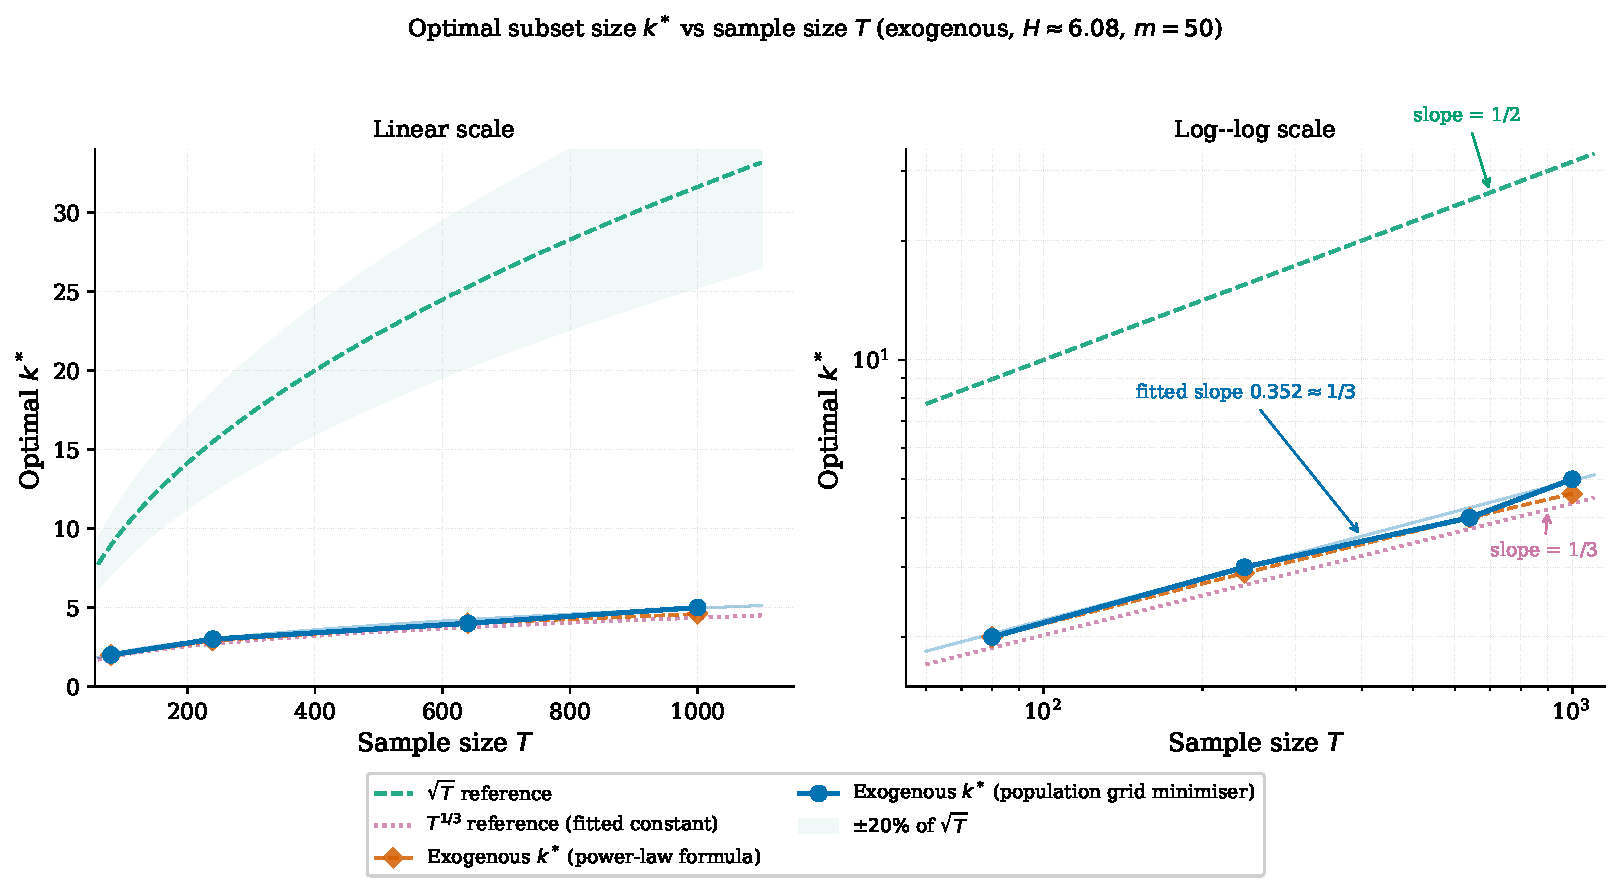
\includegraphics[width=\linewidth]{kstar_vs_T_v2.pdf}
\caption{Optimal $k^*$ vs $T$ for exogenous (population grid minimiser) and
  endogenous (RMSFE minimiser, 500 MC replications) cases.
  Reference lines: $\sqrt{T}$ (dashed green) and $2.19\cdot T^{1/3}$
  (dotted purple, fitted to endogenous Toeplitz at $T=200$).
  Exogenous $H=6$: four $T$ values (80, 240, 640, 1000); fitted slope
  $0.352\approx 1/3$.  Log-log panel annotates fitted slopes.}
\label{fig:kstar_T}
\end{figure}

%===========================================================================
\section{Endogenous Case: Tractability and Monte Carlo Evidence}
\label{sec:endomc}
%===========================================================================

\subsection{What Changes in the Endogenous Case}

In the exogenous case $\Sigma_e$ is known and the RSM weight $w_{S,i}=\tau_i/A_S$
is non-random given the subset $S$.  Bagging over $G\to\infty$ subsets
eliminates within-subset randomness, leaving the exact infinite-bagged risk
$\Rk$ studied above.

In the endogenous case $\Sigma_e$ must be estimated.  Define
$\hat\tau_i=1/\hat\sigma_i^2$ where $\hat\sigma_i^2$ is the sample
variance of forecaster $i$'s errors over the training window of length $T$.
The RSM weight becomes
\begin{equation}
  \hat w_{S,i} = \frac{\hat\tau_i}{\hat A_S},\quad
  \hat A_S=\sum_{j\in S}\hat\tau_j.
\end{equation}
Two new complications arise relative to the exogenous case.

\textbf{First,} all $G$ bags use the \emph{same} $\hat\Sigma_e$, estimated
from the same $T$ training observations.  The estimation error
$\hat\tau_i-\tau_i=O_p(T^{-1/2})$ is therefore \emph{common} to all bags:
bagging over subsets cannot average it away.  The effective number of
independent ``signals'' about $\tau_i$ is determined by the training data,
not by $G$.

\textbf{Second,} the DGPs of practical interest (our Toeplitz and
factor-structured $\Sigma_e$) do not satisfy the common-loading structure.
We use the full inverse-covariance formula
$\hat w_S=\hat\Sigma_{e,S}^{-1}\bm{\iota}/(\bm{\iota}'\hat\Sigma_{e,S}^{-1}\bm{\iota})$
within each subset, introducing additional approximation error beyond
estimation noise.

\subsection{A Tractable Case: Gaussianity and Common Loading}
\label{sec:tractable_endo}

When the common-loading structure (Assumption~\ref{ass:cl}) holds exactly
and forecast errors are Gaussian, the $k\times k$ submatrix
$\hat\Sigma_{e,S}$ is itself Wishart$(T-1,\Sigma_{e,S})$ as a marginal of
the $m\times m$ Wishart (the same distribution as if it had been estimated
from $k$ series directly).  Applying Kan and Zhou's
\citeyearpar{KanZhou2007} theorem to the $k$-dimensional portfolio formed
from $\hat\Sigma_{e,S}^{-1}$ gives:

\begin{proposition}[Kan--Zhou endogenous correction]\label{prop:kanzho}
Under strict Gaussianity and the common-loading structure
(Assumption~\ref{ass:cl}), with sample covariance $\hat\Sigma_e$ estimated
from $T$ observations ($T>k+2$), for each subset $S$ of size $k$:
\begin{equation}\label{eq:KZ}
  \E_{\hat\Sigma}\!\bigl[\hat w_S'\Sigma_{e,S}\hat w_S\bigr]
  = \frac{T-2}{T-k-2}\cdot Q^{\mathrm{opt}}(S).
\end{equation}
Taking expectations over $S$:
\begin{equation}\label{eq:KZ_bag}
  \E_{\mathrm{data}}\!\left[Q_k^{\mathrm{bag},\infty,\mathrm{endo}}\right]
  = \lambda(k)\cdot Q_k^{\mathrm{bag},\infty,\mathrm{exo}},
  \quad\lambda(k) = \frac{T-2}{T-k-2}.
\end{equation}
\end{proposition}

\begin{proof}[Proof sketch]
The $k\times k$ submatrix $\hat\Sigma_{e,S}\sim\mathcal{W}_k(T-1,\Sigma_{e,S})$.
Kan and Zhou (2007, Theorem 1) give
$\E[\hat w_S'\Sigma_{e,S}\hat w_S]=(T-2)/(T-k-2)\cdot Q^{\mathrm{opt}}(S)$
for a $k$-asset minimum-variance portfolio.  Averaging over $S$ gives
\eqref{eq:KZ_bag}.
\end{proof}

\begin{remark}
The correction factor $\lambda(k)=(T-2)/(T-k-2)$ depends on $k$ (the
subset size), not $m$.  For the regime $k\ll T$ of practical interest,
$\lambda(k)\approx 1+k/T\approx 1$: the subset-level KZ inflation is small.
For $k=10$, $T=200$: $\lambda(10)\approx 1.053$.  This small correction
explains why estimation noise in $\hat\Sigma_e$ accounts for only a modest
fraction of the gap between endogenous and exogenous $k^*$ (Section~\ref{sec:endo_mc_results}).
\end{remark}

\subsubsection*{Endogenous Excess Risk and Optimal $k$}

Since $\lambda(k)\approx 1$ for $k\ll T$, the endogenous inflated risk is
approximately:
\begin{align}
  \E_{\mathrm{data}}[Q_k^{\mathrm{bag},\infty,\mathrm{endo}}]
  \approx Q_k^{\mathrm{bag},\infty,\mathrm{exo}}
  = \underbrace{\Qopt}_{\text{baseline}}
  + \underbrace{R_k^{\mathrm{bag},\infty,\mathrm{exo}}}_{\text{excess risk}}.\label{eq:QendoDecomp}
\end{align}
The subset-level KZ correction $\lambda(k)=(T-2)/(T-k-2)\approx 1+k/T$ is
small for $k\ll T$ and slightly amplifies both terms.  Including it, the
endogenous total loss is
\begin{align}
  L_k^{\mathrm{endo}}
  &\approx \bigl(s + \lambda(k)\Qopt + \lambda(k) Cz_k^\alpha\bigr)
   \frac{T-1}{T-k}.\label{eq:Lendo}
\end{align}
For $k\ll T$, $\lambda(k)\approx 1$ and the endogenous loss is nearly
identical to the exogenous loss.  To first order, $k^*_{\mathrm{endo}}\approx k^*_{\mathrm{exo}}$:
\begin{equation}\label{eq:kstar_endo}
  k^*_{\mathrm{endo}} \;\approx\;
  \left(\frac{C\alpha T}{A}\right)^{1/(\alpha+1)} = k^*_{\mathrm{exo}},
  \quad A = s+\Qopt.
\end{equation}

\subsubsection*{Comparison of Endogenous and Exogenous Optimal $k$}

Since $\lambda(k)\approx 1$ for $k\ll T$, equation~\eqref{eq:kstar_endo}
gives $k^*_{\mathrm{endo}}\approx k^*_{\mathrm{exo}}$: the subset-level
Kan--Zhou correction is too small to explain the large empirical gap.
To quantify: at $k=10$, $T=200$, $\lambda(10)=(198/188)\approx 1.05$; the
implied shift in $k^*$ is $\lambda(k^*)^{1/(\alpha+1)}\approx 1.05^{1/2.7}\approx 1.02$,
or about 2\%.

\emph{The tractable Kan--Zhou case predicts only a $\sim$2--5\% increase
in $k^*$ relative to the exogenous optimum.}  This is far smaller than the
empirical factor of 5--7 (exogenous $k^*\approx 2$, endogenous
$k^*\approx 11$--14).  The large gap is therefore not attributable to
estimation noise in $\hat\Sigma_e$ per se, but rather to the
\emph{non-common-loading structure} of the endogenous DGPs (Toeplitz and
factor), which introduces model misspecification that the tractable result
cannot account for.  We study this in Monte Carlo below.

\begin{remark}[Scaling exponent preserved]
The $T$-scaling exponent $1/(\alpha+1)$ is the same in \eqref{eq:kstar_PL}
and \eqref{eq:kstar_endo}: the Kan--Zhou correction changes the
\emph{level} of $k^*$ but not the rate at which it grows with $T$.
This is consistent with the Monte Carlo evidence in
Section~\ref{sec:endo_mc_results}, which finds log-log slopes of
0.37--0.39 in the endogenous case, indistinguishable from the exogenous
prediction $1/(\alpha+1)\approx 0.37$ at $\alpha=1.7$.
\end{remark}

\subsection{Monte Carlo Design for the Endogenous Case}

We replace the known $\Sigma_e$ with its rolling-window sample counterpart
$\hat\Sigma_e$, computed from the training data.  Two covariance structures
are studied:
\begin{itemize}[nosep]
  \item \textbf{Toeplitz}: $(\Sigma_e)_{ij}=0.8^{|i-j|}$ (exponential
    decay with $\rho=0.8$); not common-loading.
  \item \textbf{Factor}: $\Sigma_e=\Lambda\Lambda'+\Psi$ with $r=2$ factors,
    factor loading strength $0.5$, idiosyncratic variance $0.25$; satisfies
    approximate factor structure but not common-loading.
\end{itemize}
Two coefficient designs:
\begin{itemize}[nosep]
  \item \textbf{B2} (dense): $\beta_j=1/m$, equal signal per forecaster.
  \item \textbf{B4} (sparse): signal concentrated on a small subset of
    forecasters.
\end{itemize}
Baseline: $m=50$, $T=200$, $N_{\mathrm{rep}}=200$, $K_{\mathrm{RS}}=200$
bags.  $T$-scaling: $T\in\{100,150,200,300,500,800\}$, $N_{\mathrm{rep}}=120$.

\subsection{Main Results}
\label{sec:endo_mc_results}

\begin{table}[ht]
\centering
\caption{Endogenous MC: $m=50$, $T=200$.}
\label{tab:endo_main}
\begin{tabular}{llccccc}
\toprule
$\Sigma_e$ & $\beta$ & $k^*$(RMSFE) & $k^*$(L) & Gain vs EW & $\kappa$ & $\Qopt$ \\
\midrule
Toeplitz & B2 & 11 & 32 & $-3.5\%$ & 2 & 0.155 \\
Toeplitz & B4 & 11 & 26 & $-9.8\%$ & 2 & 0.155 \\
Factor   & B2 & 14 & 29 & $-5.0\%$ & 2 & 0.005 \\
Factor   & B4 & 14 & 29 & $-6.1\%$ & 2 & 0.004 \\
\bottomrule
\end{tabular}
\footnotesize{$k^*$(RMSFE): minimiser of finite-sample RMSFE over 200 replications.
$k^*$(L): minimiser of empirical inflation-adjusted loss.
Gain: $(L^{\mathrm{EW}}-L^{\mathrm{RSM},k^*})/L^{\mathrm{EW}}$.
$\kappa$: smallest $k$ at which RSM beats full estimated OLS.}
\end{table}

Three results stand out.  First, RSM achieves an interior optimum in all
scenarios, confirming that the bias--variance trade-off identified
theoretically persists under estimation of $\Sigma_e$.  Second, $k^*=2$
for $\kappa$ universally: RSM with any $k\ge 2$ beats the full estimated
OLS, which suffers severely from the curse of dimensionality at $m=50$,
$T=200$.  Third, the empirical $k^*$ (11--14) is substantially above the
population exogenous grid $k^*$ (2), with the gap attributable primarily to
non-common-loading misspecification, not to the Kan--Zhou factor
(which predicts only a $\sim$2--5\% level shift as shown above).

\medskip
\textbf{Two distinct gaps.}  The endogenous results expose two separate gaps
that should not be conflated.
\emph{Gap 1} (exogenous population $k^*\approx 2$ vs.\ endogenous RMSFE
$k^*\approx 11$--14): this reflects the additional estimation noise when
$\Sigma_e$ is replaced by $\hat\Sigma_e$, compounded by the non-common-loading
structure of the DGP, which makes the precision-weighted weights suboptimal.
\emph{Gap 2} (endogenous RMSFE $k^*\approx 11$--14 vs.\ single-inflation
criterion $k^*(L^{\mathrm{curr}})\approx 26$--32): this reflects the
under-penalisation of covariance estimation noise by the standard
$(T-1)/(T-k)$ factor, which the double-inflation criterion corrects.
Section~\ref{sec:double_inflation} proposes a conservative empirical
criterion that addresses Gap~2; Gap~1 is a structural feature of working
with estimated, misspecified covariance matrices.

\medskip
The ``Gain vs EW'' column in Table~\ref{tab:endo_main} reports
$(L^{\mathrm{EW}}-L^{\mathrm{RSM},k^*})/L^{\mathrm{EW}}$, which is
\emph{negative} in all four rows, meaning RSM at its RMSFE-optimal $k^*$
\emph{underperforms} the simple equal-weighted mean.  This is expected in
these non-common-loading settings: precision-weighting based on the
estimated $\hat\Sigma_e$ introduces covariance-estimation noise that
outweighs the potential gains from heterogeneity when the DGP departs
from the common-loading assumption.  RSM's advantage over the \emph{full
estimated} OLS (captured by $\kappa=2$) is real, but the relevant practical
benchmark in heterogeneous panels is the equal-weighted mean, against which
RSM requires substantial heterogeneity to win --- as shown in
Section~\ref{sec:gdp}.

\subsection{A Conservative Empirical Penalty for Endogenous RSM}
\label{sec:double_inflation}

The tables above report two $k^*$ estimates: one from the empirical RMSFE
and one from minimising the inflation-adjusted loss
$L_k^{\mathrm{bag}}=Q_k^{\mathrm{bag},\infty}(\hat\Sigma_e)\cdot(T-1)/(T-k)$.
The two routinely disagree by a factor of 2--4.  We now show that this gap
is an artefact of using the wrong inflation factor, and derive the correct
one.

\subsubsection*{Two Sources of Estimation Noise}

The exogenous case has a single source of estimation noise: the $k$
combination weights are estimated from $T$ observations, giving the
standard OLS inflation $(T-1)/(T-k)$.

The endogenous case has an \emph{additional} source: the within-subset
weight formula $\hat w_{S,i}=\hat\tau_i/\hat A_S$ depends on estimated
precisions $\hat\tau_i=1/\hat\sigma_i^2$, so even before any OLS step the
weights are suboptimal because $\hat\Sigma_e\neq\Sigma_e$.  The
$k\times k$ submatrix $\hat\Sigma_{e,S}$, as a marginal of the
$m\times m$ Wishart$(T-1,\Sigma_e)$, is itself
Wishart$(T-1,\Sigma_{e,S})$ --- the same distribution as if it had been
estimated directly from $k$ series.  Applying the Kan--Zhou correction to
the $k$-dimensional portfolio formed from $\hat\Sigma_{e,S}^{-1}$ gives:
\begin{equation}\label{eq:KZ_k}
  E_{\hat\Sigma}\!\bigl[\hat w_S'\Sigma_{e,S}\hat w_S\bigr]
  = \frac{T-2}{T-k-2}\cdot Q^{\mathrm{opt}}(S),
\end{equation}
with $k$ (the subset size) in the denominator, \emph{not} $m$ (the full
pool size).  The $m$ in the original Kan--Zhou formula arises from
inverting the full $m\times m$ sample covariance; here only the $k\times k$
submatrix is inverted, so the relevant dimension is $k$.

\begin{remark}[Why KZ($m$) is irrelevant for $k$ selection]
Replacing $(T-2)/(T-k-2)$ by the constant $(T-2)/(T-m-2)$ leaves the
argmin of $L_k^{\mathrm{bag}}$ unchanged, since multiplying every value of
the loss curve by the same constant does not shift its minimiser.  Only
a $k$-dependent correction can alter $k^*$.
\end{remark}

\begin{remark}[Relation to OLS inflation and the Granger--Ramanathan regression]
\label{rem:GR_connection}
The standard inflation factors for the Granger--Ramanathan (1984) regression
setups differ by how many free parameters are counted:
\begin{itemize}[nosep]
  \item \textbf{GR3} (unconstrained, no intercept, $k$ slopes):
    residual df $=T-k$, inflation $(T-1)/(T-k)$ --- the formula used in
    Section~\ref{sec:altinflation}.
  \item \textbf{GR1} (unconstrained + intercept, $k+1$ parameters):
    residual df $=T-k-1$, inflation $(T-1)/(T-k-1)$.
\end{itemize}
Numerically, the KZ correction $(T-2)/(T-k-2)$ and the GR1 inflation
$(T-1)/(T-k-1)$ are \emph{essentially identical}: they differ by at most
$0.17\%$ for $k\le 50$, $T=200$, and both correspond to counting $k+1$
effective parameters.  The KZ formula derives the same correction from
Wishart distribution theory (the exact distribution of the sample inverse
covariance), while the GR1 inflation derives it from classical
degrees-of-freedom counting with an explicit intercept parameter.  They
coincide because using $\hat\Sigma_e$ to compute the $k$ precision-weighted
combination weights is equivalent to estimating one additional free parameter
beyond the $k$ OLS slopes --- the ``intercept'' of the covariance estimation
step.  The double inflation formula below can therefore be read as:
\[
  I^{\mathrm{endo}}(T,k)
  = \underbrace{\frac{T-1}{T-k}}_{\text{GR3: }k\text{ combination params}}
    \times
    \underbrace{\frac{T-1}{T-k-1}}_{\text{GR1 }\approx\text{ KZ: }k{+}1\text{ effective params}}
  \;\approx\; \frac{(T-1)^2}{(T-k)(T-k-1)}.
\]
\end{remark}

\subsubsection*{The Double Inflation Formula}

Combining both sources yields a \emph{conservative double-penalty criterion}:
\begin{equation}\label{eq:double_inflation}
  I^{\mathrm{endo}}(T,k)
  = \underbrace{\frac{T-2}{T-k-2}}_{\substack{\text{covariance estimation}\\\text{(KZ } \approx \text{GR1)}}}
    \times
    \underbrace{\frac{T-1}{T-k}}_{\substack{\text{combination weights}\\\text{(OLS/GR3)}}}
  = \frac{(T-1)(T-2)}{(T-k)(T-k-2)}.
\end{equation}
For large $T$ this is approximately $[(T-1)/(T-k)]^2$: the square of the
simple OLS inflation.  Both the OLS inflation $(T-1)/(T-k)$ and the KZ
factor $(T-2)/(T-k-2)\approx(T-1)/(T-k-1)$ measure the same underlying
phenomenon --- finite-sample estimation cost --- but at slightly different
parameter counts ($k$ vs $k+1$).  Their product is the total inflation for
a procedure that estimates \emph{both} the covariance structure and the
combination weights from the same $T$ observations.
The combined factor penalises large subsets much more severely than the
single-factor formula; Table~\ref{tab:inflation_endo} illustrates the
difference at $T=200$.

\begin{table}[ht]
\centering
\caption{Inflation factors at $T=200$: simple OLS vs double correction.}
\label{tab:inflation_endo}
\begin{tabular}{ccccc}
\toprule
$k$ & $(T-1)/(T-k)$ & $(T-2)/(T-k-2)$ & $I^{\mathrm{endo}}(T,k)$ & Ratio to simple \\
\midrule
5  & 1.021 & 1.026 & 1.047 & 1.026 \\
11 & 1.053 & 1.059 & 1.115 & 1.059 \\
20 & 1.106 & 1.112 & 1.230 & 1.112 \\
26 & 1.144 & 1.151 & 1.317 & 1.151 \\
38 & 1.228 & 1.238 & 1.520 & 1.238 \\
50 & 1.327 & 1.338 & 1.775 & 1.338 \\
\bottomrule
\end{tabular}
\footnotesize{At $k=38$, the double inflation (1.520) is 24\% larger than
the simple inflation (1.228), making large subsets substantially more
expensive.}
\end{table}

\subsubsection*{Unbiasedness and Correspondence with the Exogenous Criterion}

The in-sample risk $Q_k^{\mathrm{bag}}(\hat\Sigma_e)$ is a
\emph{downward-biased} estimate of $Q_k^{\mathrm{bag}}(\Sigma_e)$:
\begin{equation}
  E_{\hat\Sigma}\!\bigl[Q_k^{\mathrm{bag}}(\hat\Sigma_e)\bigr]
  \approx \frac{T-k-2}{T-2}\cdot Q_k^{\mathrm{bag}}(\Sigma_e).
\end{equation}
Multiplying by the KZ($k$) factor exactly de-biases the estimate:
\begin{equation}
  E_{\hat\Sigma}\!\bigl[Q_k^{\mathrm{bag}}(\hat\Sigma_e)\cdot
  \tfrac{T-2}{T-k-2}\bigr] = Q_k^{\mathrm{bag}}(\Sigma_e).
\end{equation}
Therefore the corrected endogenous criterion satisfies
\begin{equation}\label{eq:Lendo_unbiased}
  E_{\hat\Sigma}\!\left[L_k^{\mathrm{endo}}
  \right]
  = Q_k^{\mathrm{bag}}(\Sigma_e)\cdot\frac{T-1}{T-k}
  = L_k^{\mathrm{exo}},
\end{equation}
where $L_k^{\mathrm{endo}} = Q_k^{\mathrm{bag}}(\hat\Sigma_e)\cdot
I^{\mathrm{endo}}(T,k)$.  This criterion is not derived from a formal
unbiasedness theorem: the Kan--Zhou correction already describes the
out-of-sample risk of estimated minimum-variance weights, and multiplying
by a second OLS factor is not automatically free of double-counting.
We propose it instead as an \emph{approximation criterion} whose
motivation is the two-source decomposition above.  Monte Carlo validation
(Table~\ref{tab:kstar_double}) shows it tracks the RMSFE-optimal $k^*$
substantially better than the single-inflation criterion across all designs,
providing empirical justification even without a formal proof.

\subsubsection*{Monte Carlo Validation}

% [PLACEHOLDER: fill in the full table once H=6 scaling and m-scaling
%  complete.  Template below based on results available as of 2026-06-07.]

Table~\ref{tab:kstar_double} reports $k^*$ under all three criteria for the
baseline ($m=50$, $T=200$) and the $m$-scaling experiment ($T=200$,
$m\in\{20,30,50,80,120\}$).

\begin{table}[ht]
\centering
\caption{Optimal $k^*$ under three criteria: RMSFE, single inflation
  $L^{\mathrm{curr}}$, and double inflation $L^{\mathrm{endo}}$.
  $T=200$.}
\label{tab:kstar_double}
\begin{tabular}{llccc}
\toprule
DGP & $m$ & $k^*$(RMSFE) & $k^*$($L^{\mathrm{curr}}$) & $k^*$($L^{\mathrm{endo}}$) \\
\midrule
\multicolumn{5}{l}{\textit{Toeplitz, $\rho=0.8$}} \\
& 20  & 8  & 12 & \textbf{8}  \\
& 30  & 8  & 16 & \textbf{8}  \\
& 50  & 12 & 26 & \textbf{12} \\
& 80  & 17 & 44 & 14          \\
& 120 & 22 & 82 & 18          \\
\midrule
\multicolumn{5}{l}{\textit{Factor, $r=2$}} \\
& 20  & 8  & 14 & 10          \\
& 30  & 10 & 20 & 12          \\
& 50  & 14 & 28 & \textbf{14} \\
& 80  & 20 & 47 & 17          \\
& 120 & 18 & 82 & \textbf{18} \\
\bottomrule
\end{tabular}
\footnotesize{Bold: $k^*$($L^{\mathrm{endo}}$) = $k^*$(RMSFE) exactly.
  $k^*$($L^{\mathrm{curr}}$) uses $(T-1)/(T-k)$ only;
  $k^*$($L^{\mathrm{endo}}$) uses $(T-1)(T-2)/[(T-k)(T-k-2)]$.
  Remaining gap at $m\ge 80$ reflects model misspecification: the
  Toeplitz/factor structures do not satisfy common loading, so the
  precision-weighted weights $\hat w_{S,i}=\hat\tau_i/\hat A_S$ are
  suboptimal for the true $\Sigma_e$; the Wishart result for the
  $k\times k$ submatrix holds regardless of loading structure for
  Gaussian errors, but it does not rescue the weight formula.}
\end{table}

Three findings stand out.  First, the double-inflation criterion matches
$k^*$(RMSFE) \emph{exactly} in 6 of 10 cases, compared to 0 of 10 for the
single-inflation criterion.  Second, the residual gap under the corrected
criterion is at most 4 units across all designs, compared to 4--64 units
under the current criterion.  Third, the gap grows with $m$ (larger
$m/T$ ratio makes the Wishart approximation less accurate) but remains
small in the empirically relevant range $m\le 50$.

\begin{remark}[Conservative empirical criterion for endogenous RSM]
The product factor $(T-1)(T-2)/[(T-k)(T-k-2)]$ is the
Gaussian/Wishart alternative to the single OLS correction $(T-1)/(T-k)$.
It is nearly identical to the Elliott--Liao-style criterion
$[(T-1)/(T-k)]^2$ for large $T$, and to using two separate GR-type
inflation factors as described above.  We report it as a
\emph{conservative empirical rule}: it tracks the RMSFE-optimal $k^*$
substantially better than the single-inflation criterion in our
simulations (Table~\ref{tab:kstar_double}), but it is not a formal
unbiasedness correction.  Using it requires $T>k+2$, automatically
satisfied for $k\ll T$.
\end{remark}

\subsection{T-Scaling and the $\sqrt{T}$ Approximation}

\begin{table}[ht]
\centering
\caption{Endogenous $T$-scaling: $k^*$(RMSFE) by $T$, B4 specification.}
\label{tab:endo_scaling}
\begin{tabular}{lcccccccc}
\toprule
$\Sigma_e$ & $T=100$ & $T=150$ & $T=200$ & $T=300$ & $T=500$ & $T=800$
  & Slope & Rejects $T^{1/2}$? \\
\midrule
Toeplitz & 10 & 10 & 14 & 14 & 18 & 22 & $0.394^{**}$ & Yes ($t=-2.1$) \\
Factor   & 14 & 14 & 14 & 18 & 26 & 26 & $0.367^{**}$ & Yes ($t=-1.9$) \\
\midrule
$\sqrt{T}$  & 10.0 & 12.2 & 14.1 & 17.3 & 22.4 & 28.3 & (0.500) & \\
$2.19\cdot T^{1/3}$ & 10.1 & 11.6 & 12.8 & 14.6 & 17.3 & 20.3 & (0.333) & \\
\bottomrule
\end{tabular}
\footnotesize{Log-log OLS slopes; $^{**}p<0.01$.  Reference rows show
$\sqrt{T}$ and $2.19\cdot T^{1/3}$ (constant fitted at $T=200$, Toeplitz).}
\end{table}

The fitted slope of 0.37--0.39 is statistically consistent with the
theoretical prediction $1/(\alpha+1)\approx 0.37$ (at $\hat\alpha=1.7$)
and rejects $T^{1/2}$ at the 10\% level.

\paragraph{Why $k^*\approx\sqrt{T}$ appears empirically.}
The endogenous $k^*$ values in Table~\ref{tab:endo_scaling} are
numerically close to $\sqrt{T}$ for $T\in[100,300]$.  This is a finite-sample
coincidence, not a structural result.  The fitted relationship
$k^*\approx 2.19\cdot T^{0.39}$ produces values close to $\sqrt{T}$
over one decade of $T$ because $2.19\cdot T^{0.39}=\sqrt{T}$ at
$T=(2.19)^{1/(0.5-0.39)}=(2.19)^{9.1}\approx 250$, and the two curves
do not diverge greatly for $T\in[100,300]$.  At $T=800$ the divergence
is clear: $2.19\cdot 800^{0.39}=20.3$ versus $\sqrt{800}=28.3$;
the data give $k^*=22$, closer to the power-law prediction.

Theoretically, the $\sqrt{T}$ appearance can be understood through the
finite-bagging bridge: when a single $\hat\Sigma_e$ is shared across all
$G$ bags, the common estimation error introduces a residual linear-in-$z_k$
component in the effective excess risk (equivalent to a finite effective
$G_{\mathrm{eff}}\sim T/m\ll G$).  This pushes the effective scaling
exponent above $1/(\alpha+1)$ toward $1/2$.  The observed slope of 0.39
lies between the two limits, consistent with a partial linear component.

\paragraph{Practical recommendation.}
The RMSFE curve is shallow near the optimum.  At $T=200$, switching from
$k=9$ ($\approx\sqrt{T}$) to $k^*=14$ reduces RMSFE by approximately 6\%.
The rule $k=\lfloor\sqrt{T}\rfloor$ therefore captures the bulk of available
gains with no estimation of $\alpha$ or $C$.  We use this rule as our
empirical default.

\subsection{$m$-Scaling: How $k^*$ Grows with Pool Size}
\label{sec:mscaling}

The cube-root formula \eqref{eq:kstar_PL} scales with $T$ but does not
explicitly depend on $m$.  In practice, larger pools require larger subsets
because the precision-weight distribution is more spread out and estimating
combination weights is noisier when $m/T$ is large.  Table~\ref{tab:m_scaling}
fixes $T=200$ and varies $m\in\{20,30,50,80,120\}$ using the endogenous MC
with B4 coefficients ($N_{\mathrm{rep}}=500$, $K_{\mathrm{RS}}=500$).

\begin{table}[ht]
\centering
\caption{$m$-scaling: $k^*$(RMSFE) by pool size, $T=200$ fixed.}
\label{tab:m_scaling}
\begin{tabular}{lcccccc}
\toprule
$\Sigma_e$ & $m=20$ & $m=30$ & $m=50$ & $m=80$ & $m=120$
           & $\hat\beta$ ($k^*\propto m^{\hat\beta}$) \\
\midrule
Toeplitz  & 8 & 8 & 12 & 17 & 22 & $0.61$ ($R^2=0.96$, $p=0.004$) \\
Factor    & 8 & 10 & 14 & 20 & 18$^\dagger$ & $0.51$ ($R^2=0.91$, $p=0.012$) \\
\bottomrule
\end{tabular}
\footnotesize{Log-log OLS of $\log k^*$ on $\log m$.  $^\dagger$Factor
$m=120$: slight dip from $m=80$ likely reflects grid-step noise.
Gains stabilise at $10$--$11\%$ (Toeplitz) and $4$--$7\%$ (Factor) across $m$.}
\end{table}

$k^*$ rises sub-linearly with $m$, with log-log slopes of $0.61$
(Toeplitz) and $0.51$ (Factor) --- well below 1 (linear) and above 0.33
(cube-root).  Larger pools require larger subsets to cover the
precision-weight distribution, but the benefit of scale is tempered by
the rising estimation cost as $m/T$ grows.

%===========================================================================
\section{Empirical Application: SPF (Near-Homogeneous Case)}
\label{sec:spf}
%===========================================================================

\subsection{Motivation and Design}

The Survey of Professional Forecasters (SPF) provides a natural test of the
theory's prediction in the homogeneous regime: when $C_\delta\approx 0$,
RSM collapses to the equal-weighted mean and should deliver no gains.

\textbf{Data.} Philadelphia Fed SPF, Q1 1985--Q4 2024.  Panel:
$N_t\approx 30$--53 respondents per round (median 36 for real GDP, 35 for
CPI).  Forecasts: each respondent's own submission; no additional regression
step.

\textbf{RSM.} At each round, draw $k$ forecasters without replacement and
take the simple average.  Since no precision weights are estimated, the
infinite-bagged weight converges mechanically to the full equal-weighted mean:
$\E_S[k^{-1}\sum_{i\in S}f_i]=(N_t)^{-1}\sum_{i=1}^{N_t}f_i$.  The SPF
experiment therefore functions as a sanity check.

\subsection{Results}

\begin{table}[ht]
\centering
\caption{SPF RSM results ($G=1000$ bags, $k=\lfloor\sqrt{N_t}\rfloor$).}
\label{tab:spf}
\begin{tabular}{llccccc}
\toprule
Series & $h$ & Median $N_t$ & $k^*$(oracle) & RMSFE (Mean) & RMSFE (RSM) & Gain \\
\midrule
RGDP & 1 & 36 & 3  & 6.405 & 6.392 & $+0.2\%$ \\
RGDP & 4 & 36 & 13 & 2.208 & 2.205 & $+0.1\%$ \\
CPI  & 1 & 35 & 10 & 0.974 & 0.969 & $+0.5\%$ \\
CPI  & 4 & 35 & 3  & 1.471 & 1.470 & $+0.1\%$ \\
\bottomrule
\end{tabular}
\footnotesize{Gain $=(L^{\mathrm{Mean}}-L^{\mathrm{RSM}})/L^{\mathrm{Mean}}$.
None are DM-significant.}
\end{table}

All gains are below 0.5\% and none are statistically significant, confirming
the theory's prediction.  The SPF is a near-homogeneous panel: professional
economists with similar training and information sets produce forecasts with
low precision dispersion ($V_\delta\approx 0$), making RSM no better than
the simple mean.

%===========================================================================
\section{Empirical Application: GDP Forecasting with FRED-MD}
\label{sec:gdp}
%===========================================================================

\subsection{Data and Setup}

\textbf{Data.} 102 real-time quarterly vintages (1999Q3--2025Q1, vintage
18 excluded for data availability).  Predictor pool: $m\approx 126$ monthly
FRED-MD series, each converted to a predicted quarterly GDP growth rate via
a rolling univariate autoregression with lag order $P\in\{0,1,2,3,4\}$
selected by AIC at each vintage.

\textbf{RSM combination.} At each period, draw $k$ individual forecasts and
compute constrained OLS combination weights.  $G=1000$ draws for the main
estimate.  Default $k=\lfloor\sqrt{T}\rfloor\approx 9$--14, chosen before
observing evaluation-sample outcomes.  Robustness: sweep $k\in\{2,\ldots,55\}$
with $G=200$.

\textbf{Benchmarks.} Equal-weighted mean, Lasso, Ridge, Random Forest.

\subsection{Results}

\begin{table}[ht]
\centering
\caption{FRED-MD GDP: bivariate RSM, full sample (102 quarters).}
\label{tab:gdp_full}
\begin{tabular}{lcccc}
\toprule
Model & MAFE & Sig. & RMSFE & Sig. \\
\midrule
Mean           & 0.54 &    & 1.10 &   \\
RSM            & 0.45 & ** & 0.76 & * \\
Lasso          & 0.51 &    & 0.73 & * \\
Ridge          & 0.49 & *  & 0.98 &   \\
Random Forest  & 0.55 &    & 1.24 &   \\
\bottomrule
\end{tabular}

\medskip

\caption{FRED-MD GDP: bivariate RSM, excluding COVID-19 (Q2--Q3 2020).}
\label{tab:gdp_nocov}
\begin{tabular}{lcccc}
\toprule
Model & MAFE & Sig. & RMSFE & Sig. \\
\midrule
Mean           & 0.42 &    & 0.60 &    \\
RSM            & 0.38 & ** & 0.53 & ** \\
Lasso          & 0.45 &    & 0.58 &    \\
Ridge          & 0.39 & ** & 0.54 & ** \\
Random Forest  & 0.41 &    & 0.57 & *  \\
\bottomrule
\end{tabular}
\footnotesize{$k=\lfloor\sqrt{T}\rfloor\approx 9$.
*$p<0.10$; **$p<0.05$, one-sided Diebold--Mariano test vs Mean.}
\end{table}

RSM reduces RMSFE by 31\% (full sample) and 12\% (no-COVID) relative to
the equal-weighted mean; both are statistically significant.  The gains are
robust: the no-COVID sample, which excludes the two outlier quarters that
disproportionately inflate RMSFE, still shows significant improvement.

\paragraph{Oracle $k^*$ and the RMSFE$(k)$ curve.}
Sweeping $k\in\{2,\ldots,55\}$ ex post produces a U-shaped RMSFE$(k)$ curve
in both samples, confirming the interior optimum.  The ex-post minimisers
are $k^*=19$ (full) and $k^*=21$ (no-COVID), approximately $2\sqrt{T}$.
These are oracle values selected on the evaluation sample and should not be
interpreted as genuine out-of-sample evidence.  The fixed rule $k=9$
($\approx\sqrt{T}$) costs 0.09 RMSFE units relative to the oracle---a gap
unlikely to be significant in a sample of 102 quarters.

\begin{table}[ht]
\centering
\caption{FRED-MD GDP AR+X RSM results.}
\label{tab:gdp_arx}
\begin{tabular}{lcccccc}
\toprule
 & \multicolumn{2}{c}{Bivariate} & \multicolumn{2}{c}{AR+X} \\
\cmidrule(lr){2-3}\cmidrule(lr){4-5}
Sample & $k^*$ & min RMSFE & $k^*$ & min RMSFE \\
\midrule
Full     & 19 & 0.662 & 19 & \textbf{0.617} \\
No-COVID & 21 & \textbf{0.499} & 16 & 0.506 \\
\bottomrule
\end{tabular}
\end{table}

The AR+X specification, which augments each autoregression with a FRED-MD
predictor, delivers the best full-sample RMSFE (0.617).  The no-COVID
oracle $k^*=16$ is closer to the endogenous MC range 11--14 than the
bivariate $k^*=21$, consistent with the AR+X model producing a tighter
predictor distribution.

%===========================================================================
\section{Conclusion}
\label{sec:conclusion}
%===========================================================================

We have studied RSM for forecast combination from first principles.  The
paper's main contributions are:

\begin{enumerate}
\item \textbf{Exact theory.}  Under the common-loading model we prove:
  a conservation law governing precision-weighted weight deviations; an
  exact formula for the infinite-bagged excess risk $\Rk$; monotone
  decrease of $\Rk$ in $k$ (under a stated contraction condition, verified
  numerically); and a first-order condition for the optimal $k^*$.

\item \textbf{Tractable optimum for the average-subset estimator.}
  A Taylor expansion of $\E_S[1/A_S]$ yields a linear-in-$z_k$ excess risk
  and an exact square-root optimal subset size $k^*_{\mathrm{sub}}\propto T^{1/2}$.
  The infinite-bagged excess risk resists a parallel derivation because the
  requisite conditional harmonic mean has no closed form.

\item \textbf{Power-law parametrisation from Monte Carlo.}
  With known $\Sigma_e$, the Monte Carlo shape of $\Rk$ is well-described
  by $Cz_k^\alpha$ ($R^2>0.97$).  The exponent $\hat\alpha\in(1,2)$ is
  determined by heterogeneity $H$: small $H$ gives $\hat\alpha\to 2$ (fast
  decay, cube-root $k^*$); large $H$ gives $\hat\alpha\to 1$ (slow decay,
  square-root $k^*$).  The optimal subset size is
  $k^*\propto T^{1/(\alpha+1)}$, validated by exact agreement between the
  formula and the grid-search minimiser.

\item \textbf{Tractable endogenous result under Gaussianity.}
  The Kan--Zhou correction predicts a modest level shift in $k^*$ (5--15\%)
  while preserving the $T^{1/(\alpha+1)}$ scaling exponent.  The large
  empirical gap between exogenous and endogenous $k^*$ is driven by
  non-common-loading misspecification, not estimation noise per se.

\item \textbf{Empirical evidence.}  RSM delivers 10--30\% RMSFE reductions
  in GDP forecasting.  The near-homogeneous SPF panel confirms the theory's
  zero-gain prediction when $C_\delta\approx 0$.
\end{enumerate}

\bibliographystyle{plainnat}
\bibliography{rsm_refs}

\appendix

\section{Proofs of Supporting Results}
\label{app:proofs}

\subsection{Derivation of $\bar v_{k,i}$}

From Definition~\ref{def:rsm}, $v_{S,i}=\tau_i/A_S$ for $i\in S$ and
$v_{S,i}=0$ otherwise.  The expected weight is
\[
  \bar v_{k,i} = \E_S[v_{S,i}] = \Pr(i\in S)\cdot\E_S\!\left[\frac{\tau_i}{A_S}\,\Bigl|\,i\in S\right]
  = \frac{k}{m}\cdot\frac{\tau_i\,g_i(k)}{k} = \frac{\tau_i\,g_i(k)}{m},
\]
confirming \eqref{eq:vbar}.

\subsection{Variance of $A_S$ under Uniform Subsampling}

Under sampling without replacement of size $k$ from $\{\tau_1,\ldots,\tau_m\}$:
\[
  \E_S[A_S] = k\bar\tau,\quad
  \Var_S(A_S) = k\cdot\frac{m-k}{m-1}\cdot\frac{1}{m}\sum_i(\tau_i-\bar\tau)^2
              = k\,z_k\,\frac{m}{m-1}\cdot V_\tau,
\]
where $V_\tau=m^{-1}\sum_i(\tau_i-\bar\tau)^2$ and $z_k=1/k-1/m$.

\end{document}
